\captionsetup[figure]{font=footnotesize,labelfont=footnotesize}

\section{Amazon Reviews -- Drift Matrices}
\label{app:amazon_reviews}

\noindent The cohort-mean and per-model deviation matrices shown here, and the in-distribution, future, and decay quantities tabulated below, are defined in Section~\ref{subsec:drift_summary}.

\begin{figure}[H]
\centering
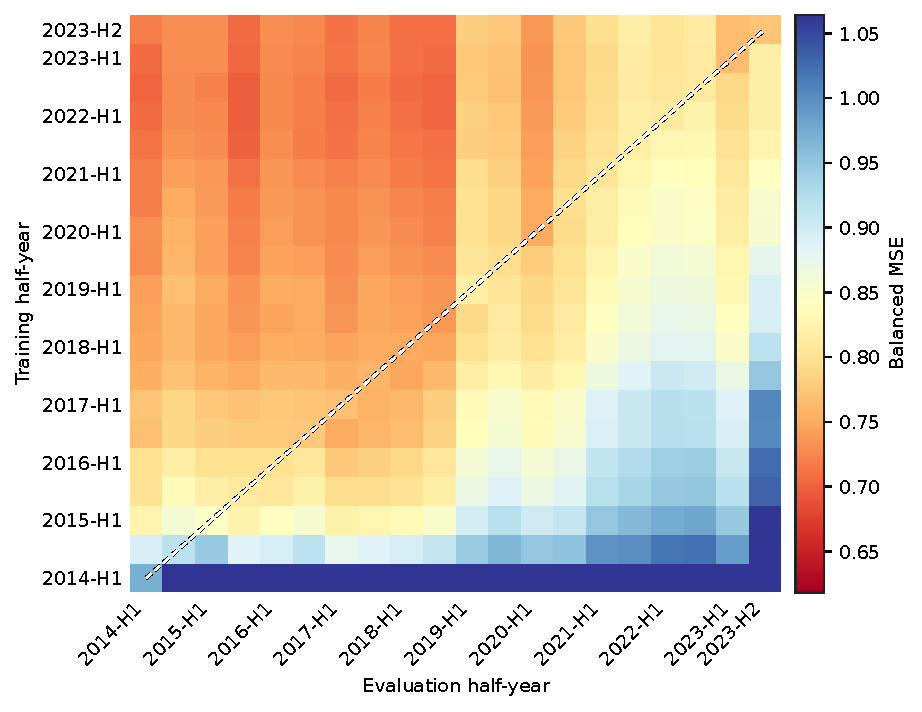
\includegraphics[width=0.5\textwidth]{plots_experiments/amazon_reviews/mean_mse_matrix.pdf}
\caption{Cohort-mean Balanced MSE matrix $\bar{M}$ over the Amazon Reviews models. Cell $(i,j)$ is the mean across those models of the score from training through slice $i$ and evaluating on slice $j$.}
\label{fig:amazon_reviews_mean_matrix}
\end{figure}

\subsection{Model Roster}

\noindent
\begin{minipage}[t]{0.49\linewidth}
\centering
\footnotesize
\captionof{table}{Amazon Reviews: models trained from scratch.}
\label{tab:amazon_reviews_roster}
\resizebox{\ifdim\width>\linewidth \linewidth\else\width\fi}{!}{%
\begin{tabular}{l l rr}
\toprule
Model & Family & Trainable & Total \\
\midrule
TX-S & Transformer & 83k & 124.7M \\
TextCNN-S & TextCNN & 88k & 124.7M \\
FFN-S & FFN & 99k & 124.7M \\
BiGRU-S & Recurrent & 99k & 124.7M \\
FFN-M & FFN & 394k & 125.0M \\
TextCNN-M & TextCNN & 461k & 125.1M \\
TX-M & Transformer & 493k & 125.1M \\
BiLSTM-M & Recurrent & 536k & 125.2M \\
FFN-L & FFN & 1.6M & 126.2M \\
TX-L & Transformer & 1.9M & 126.5M \\
TextCNN-L & TextCNN & 1.9M & 126.6M \\
BiLSTM-Attn-L & Recurrent & 2.2M & 126.8M \\
\bottomrule
\end{tabular}}
\end{minipage}
\hfill
\begin{minipage}[t]{0.49\linewidth}
\centering
\footnotesize
\captionof{table}{Amazon Reviews: frozen pretrained encoders, with trainable head and total parameters.}
\label{tab:amazon_reviews_roster_frozen}
\resizebox{\ifdim\width>\linewidth \linewidth\else\width\fi}{!}{%
\begin{tabular}{l l rr}
\toprule
Model & Family & Trainable & Total \\
\midrule
DistilBERT & Frozen & 769 & 66.4M \\
ELECTRA & Frozen & 769 & 108.9M \\
BERT & Frozen & 769 & 109.5M \\
MPNet & Frozen & 769 & 109.5M \\
RoBERTa & Frozen & 769 & 124.6M \\
ModernBERT & Frozen & 769 & 149.0M \\
DeBERTa-v3 & Frozen & 769 & 183.8M \\
\bottomrule
\end{tabular}}
\end{minipage}


\subsection{FFN}

\begin{figure}[H]
\centering
\begin{subfigure}[t]{0.49\textwidth}\centering
    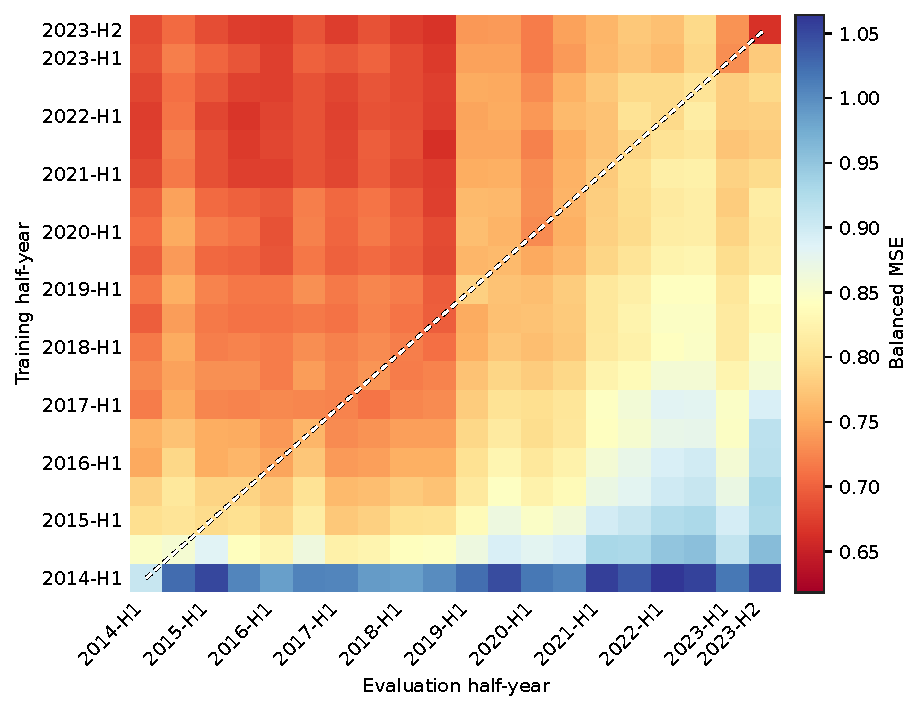
\includegraphics[width=0.49\linewidth]{plots_experiments/amazon_reviews/raw/FFN-S_drift_matrix.pdf}\hfill
    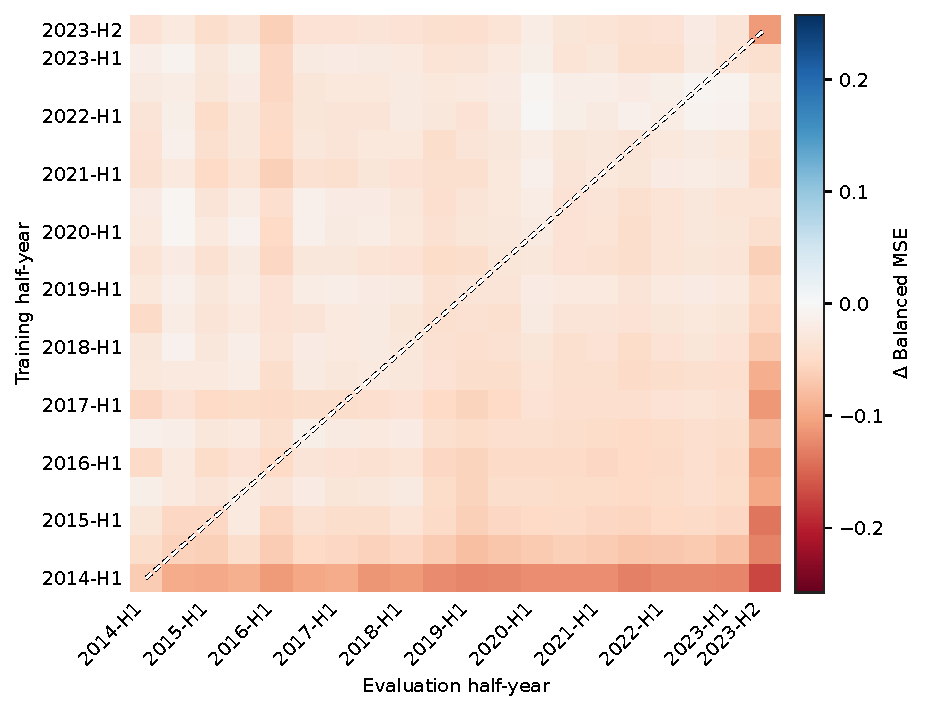
\includegraphics[width=0.49\linewidth]{plots_experiments/amazon_reviews/deviation/FFN-S_deviation.pdf}
    \caption{FFN-S}
    \label{fig:amazon_reviews_FFN_S}
\end{subfigure}
\hfill
\begin{subfigure}[t]{0.49\textwidth}\centering
    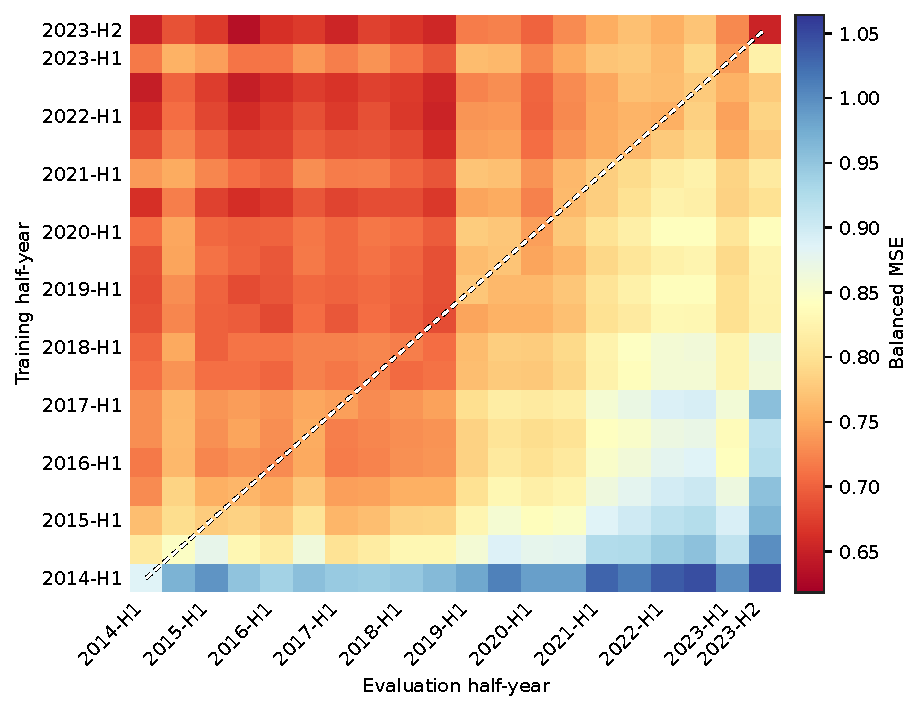
\includegraphics[width=0.49\linewidth]{plots_experiments/amazon_reviews/raw/FFN-M_drift_matrix.pdf}\hfill
    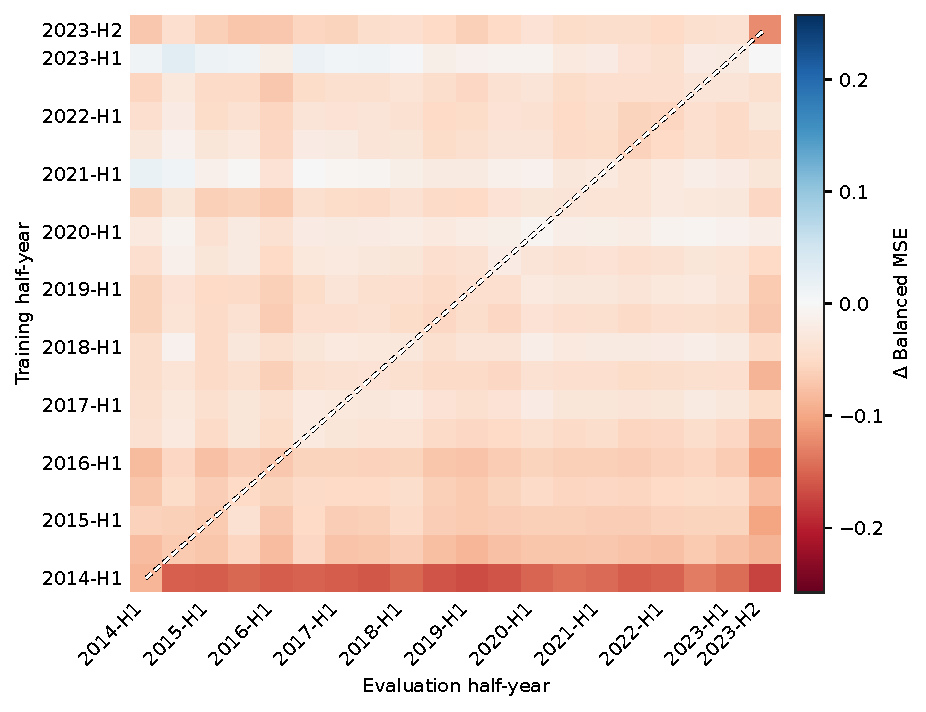
\includegraphics[width=0.49\linewidth]{plots_experiments/amazon_reviews/deviation/FFN-M_deviation.pdf}
    \caption{FFN-M}
    \label{fig:amazon_reviews_FFN_M}
\end{subfigure}

\begin{subfigure}[t]{0.49\textwidth}\centering
    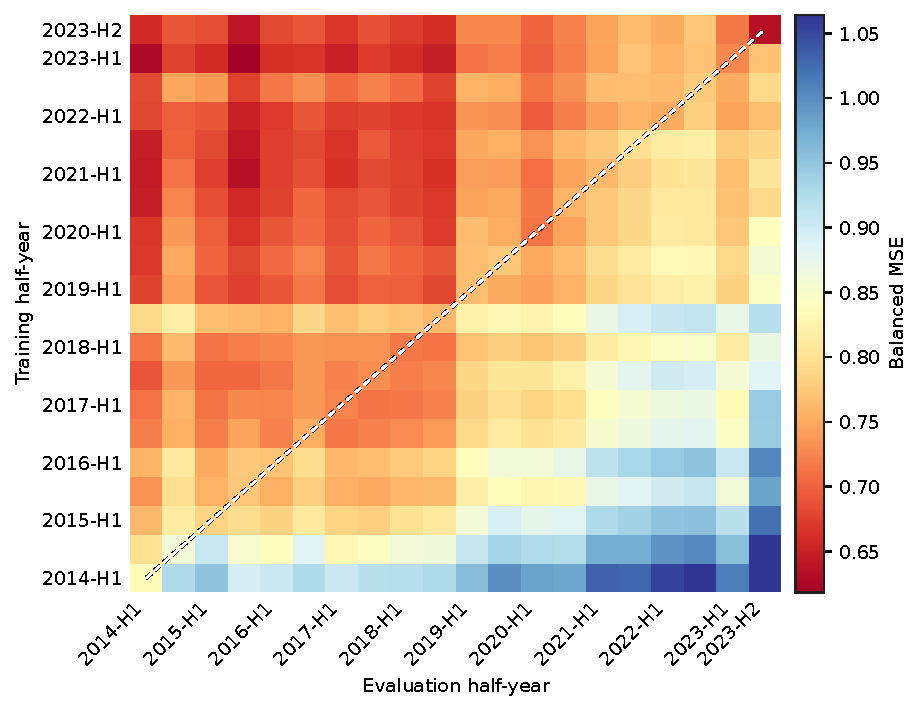
\includegraphics[width=0.49\linewidth]{plots_experiments/amazon_reviews/raw/FFN-L_drift_matrix.pdf}\hfill
    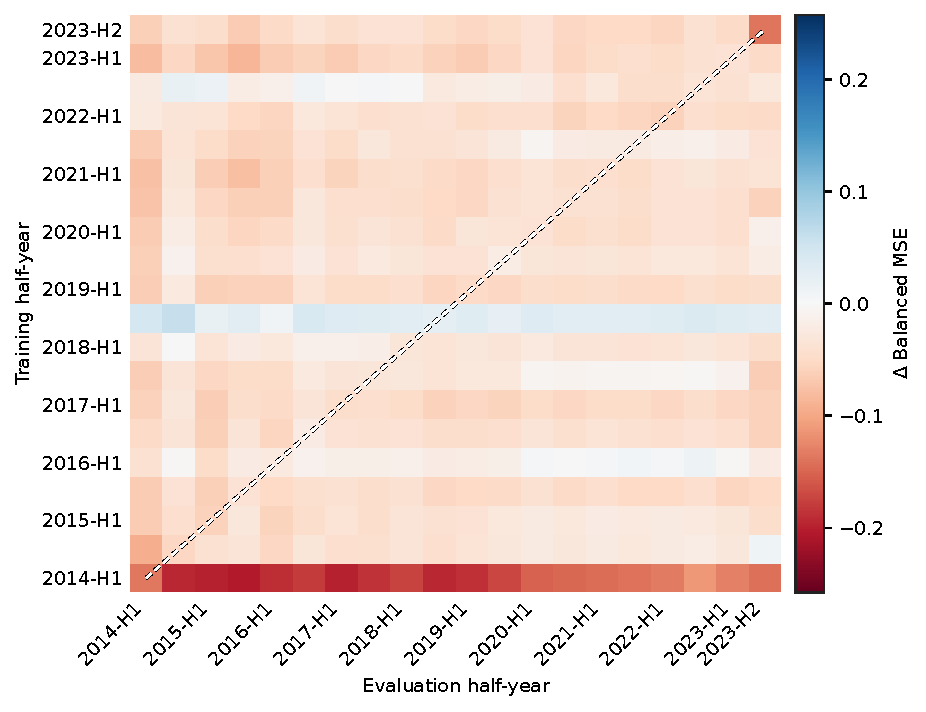
\includegraphics[width=0.49\linewidth]{plots_experiments/amazon_reviews/deviation/FFN-L_deviation.pdf}
    \caption{FFN-L}
    \label{fig:amazon_reviews_FFN_L}
\end{subfigure}
\caption{FFN models: Balanced MSE drift matrix $M^{(m)}$ and deviation from the cohort mean $\Delta^{(m)} = M^{(m)} - \bar{M}$ for each model, shown on a sequential and a zero-centred diverging scale, respectively.}
\label{fig:amazon_reviews_family_text_ffn_regression}
\end{figure}

\subsection{TextCNN}

\begin{figure}[H]
\centering
\begin{subfigure}[t]{0.49\textwidth}\centering
    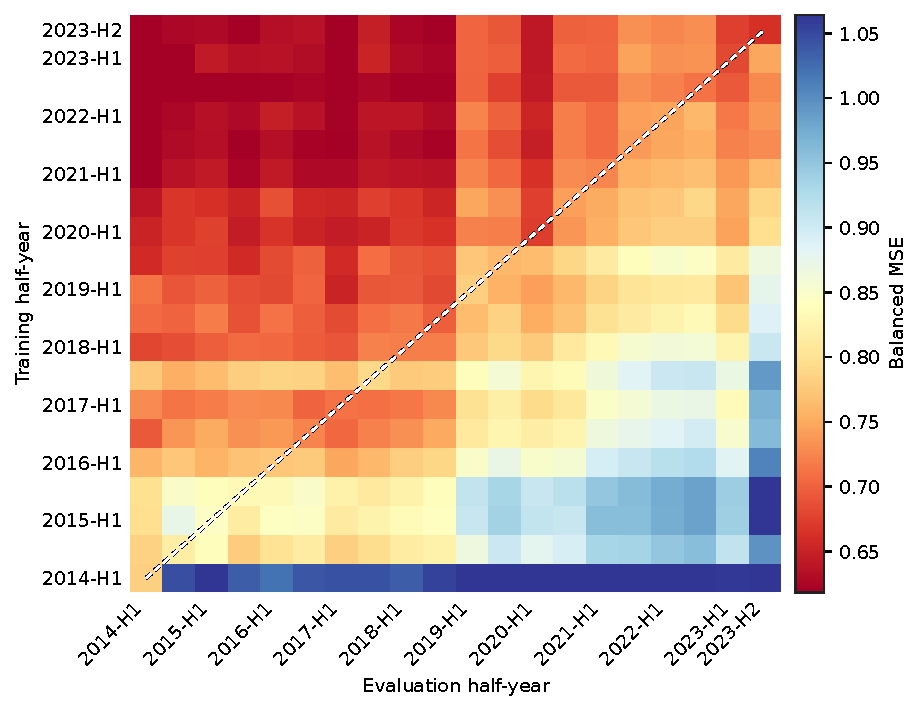
\includegraphics[width=0.49\linewidth]{plots_experiments/amazon_reviews/raw/TextCNN-S_drift_matrix.pdf}\hfill
    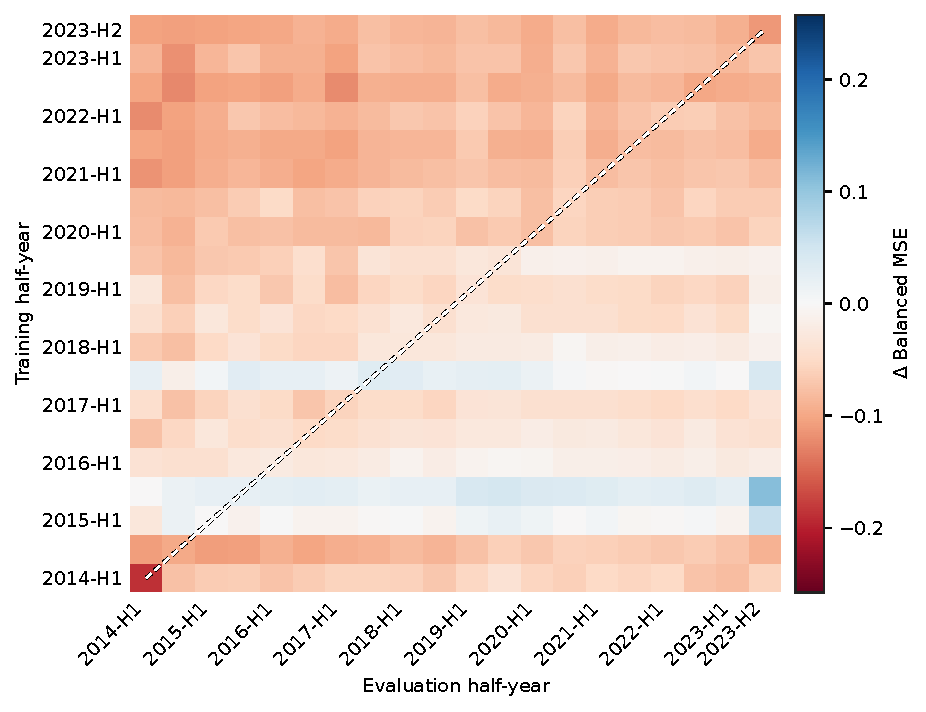
\includegraphics[width=0.49\linewidth]{plots_experiments/amazon_reviews/deviation/TextCNN-S_deviation.pdf}
    \caption{TextCNN-S}
    \label{fig:amazon_reviews_TextCNN_S}
\end{subfigure}
\hfill
\begin{subfigure}[t]{0.49\textwidth}\centering
    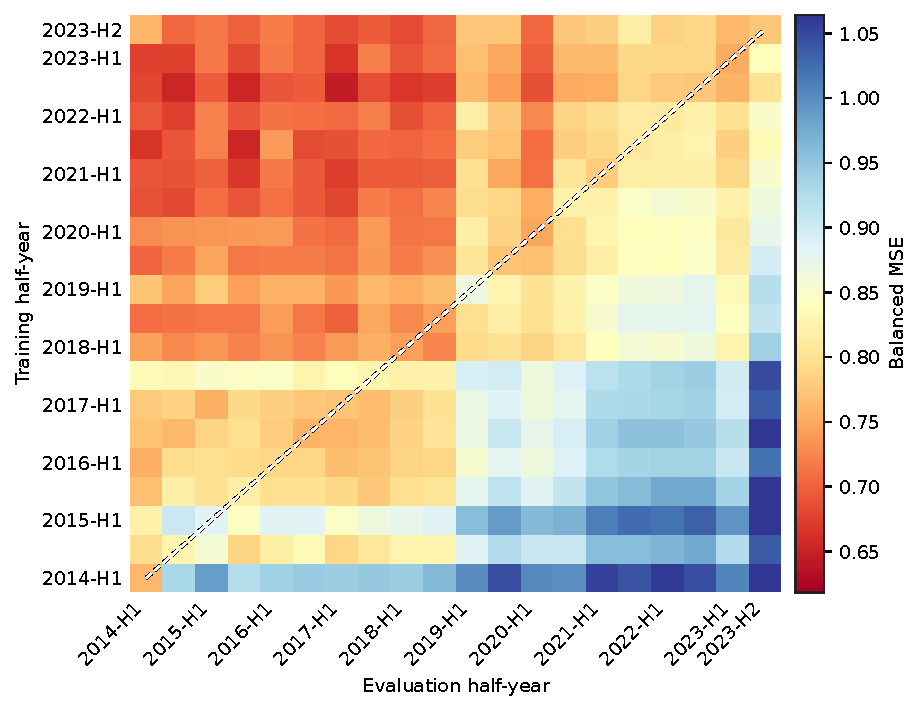
\includegraphics[width=0.49\linewidth]{plots_experiments/amazon_reviews/raw/TextCNN-M_drift_matrix.pdf}\hfill
    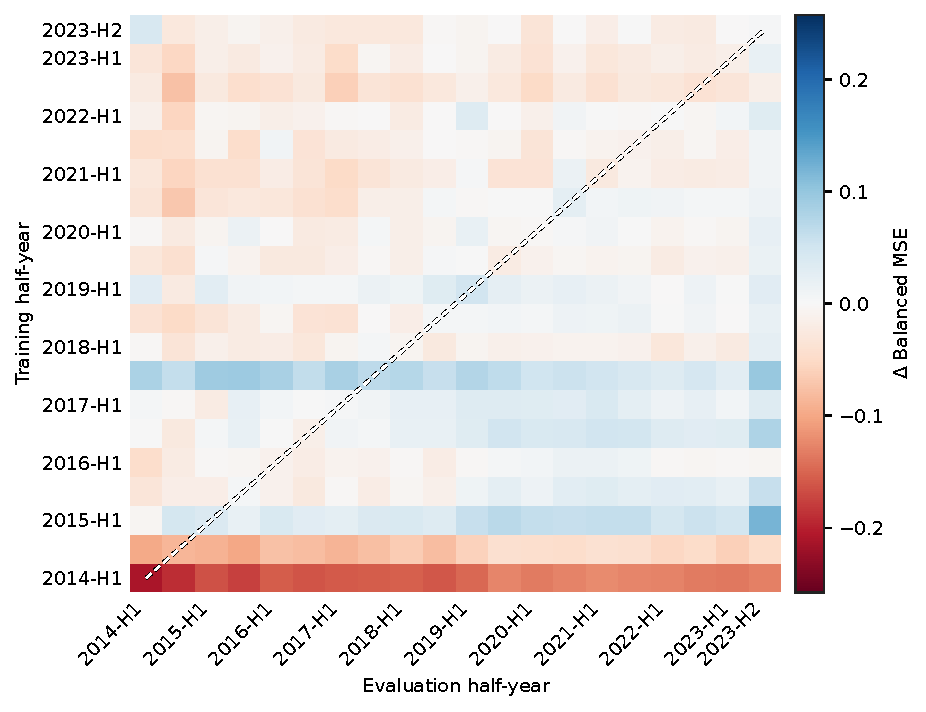
\includegraphics[width=0.49\linewidth]{plots_experiments/amazon_reviews/deviation/TextCNN-M_deviation.pdf}
    \caption{TextCNN-M}
    \label{fig:amazon_reviews_TextCNN_M}
\end{subfigure}

\begin{subfigure}[t]{0.49\textwidth}\centering
    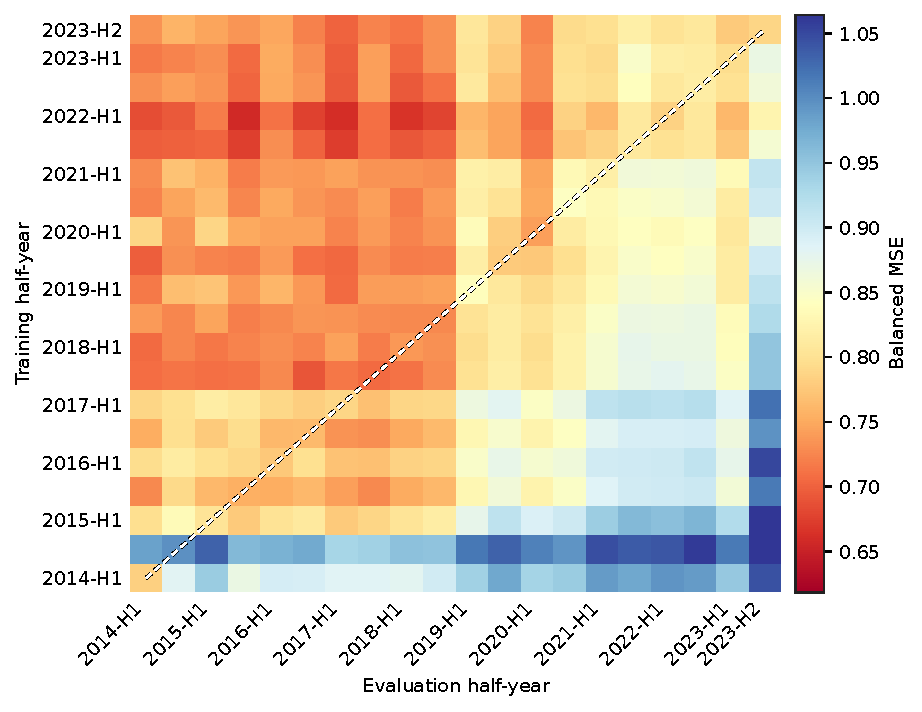
\includegraphics[width=0.49\linewidth]{plots_experiments/amazon_reviews/raw/TextCNN-L_drift_matrix.pdf}\hfill
    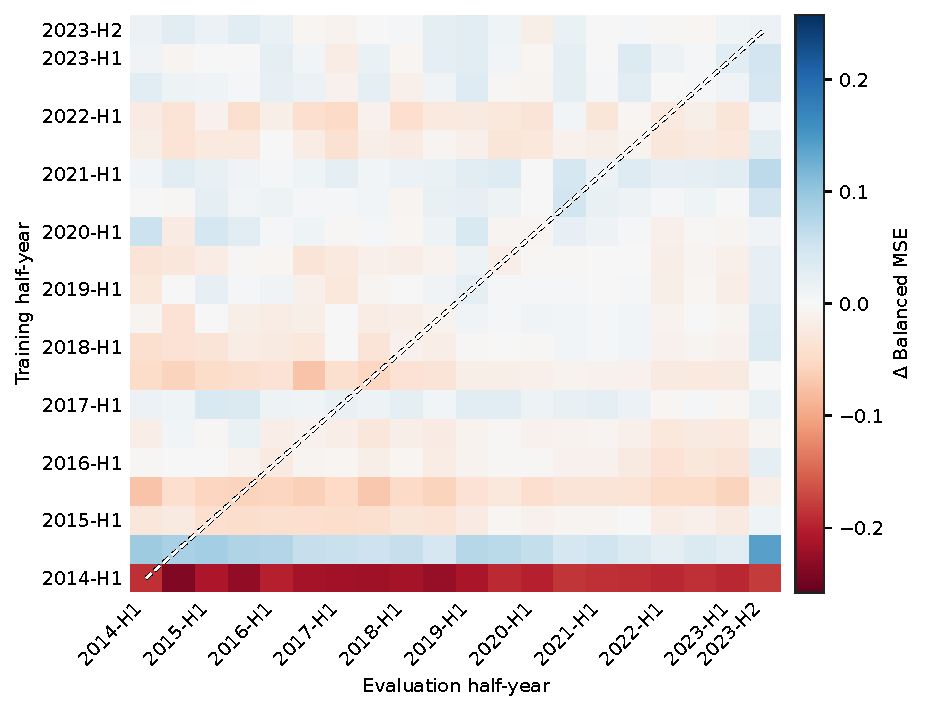
\includegraphics[width=0.49\linewidth]{plots_experiments/amazon_reviews/deviation/TextCNN-L_deviation.pdf}
    \caption{TextCNN-L}
    \label{fig:amazon_reviews_TextCNN_L}
\end{subfigure}
\caption{TextCNN models: Balanced MSE drift matrix $M^{(m)}$ and deviation from the cohort mean $\Delta^{(m)} = M^{(m)} - \bar{M}$ for each model, shown on a sequential and a zero-centred diverging scale, respectively.}
\label{fig:amazon_reviews_family_text_textcnn_regression}
\end{figure}

\subsection{Recurrent}

\begin{figure}[H]
\centering
\begin{subfigure}[t]{0.49\textwidth}\centering
    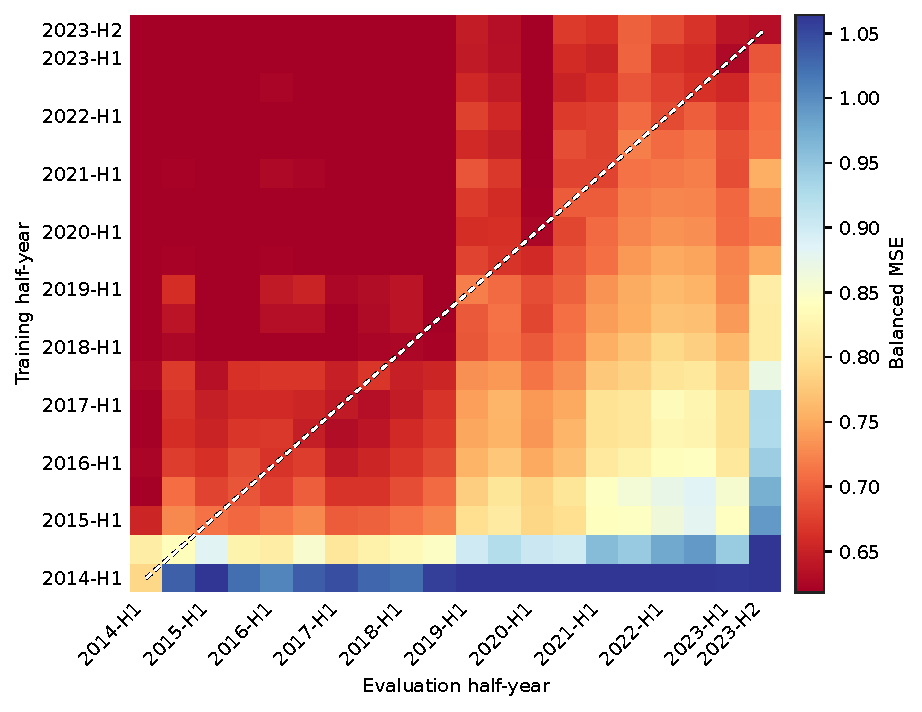
\includegraphics[width=0.49\linewidth]{plots_experiments/amazon_reviews/raw/BiGRU-S_drift_matrix.pdf}\hfill
    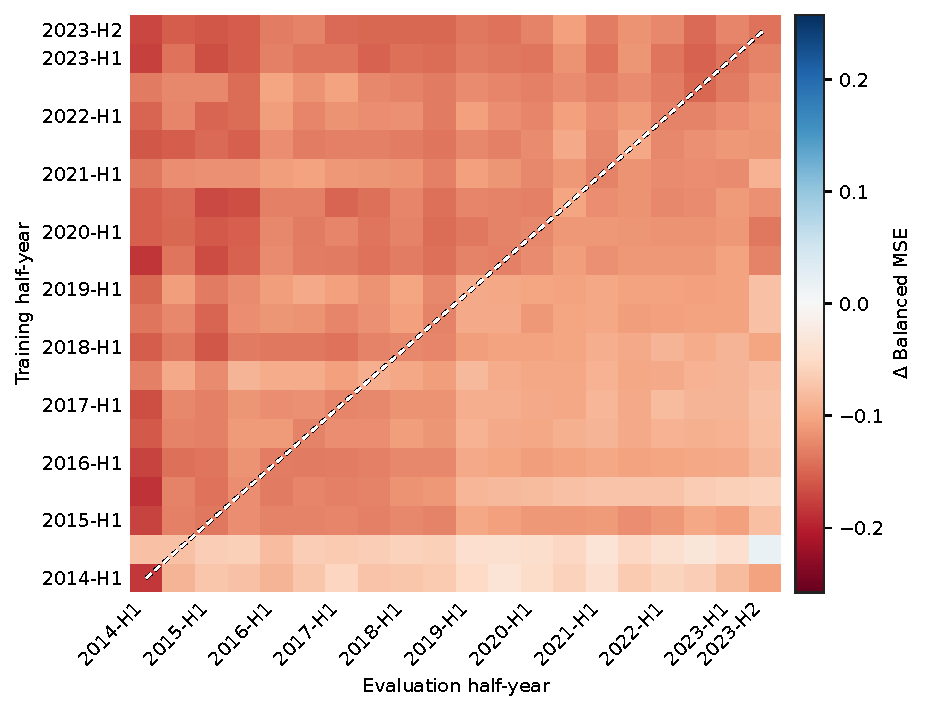
\includegraphics[width=0.49\linewidth]{plots_experiments/amazon_reviews/deviation/BiGRU-S_deviation.pdf}
    \caption{BiGRU-S}
    \label{fig:amazon_reviews_BiGRU_S}
\end{subfigure}
\hfill
\begin{subfigure}[t]{0.49\textwidth}\centering
    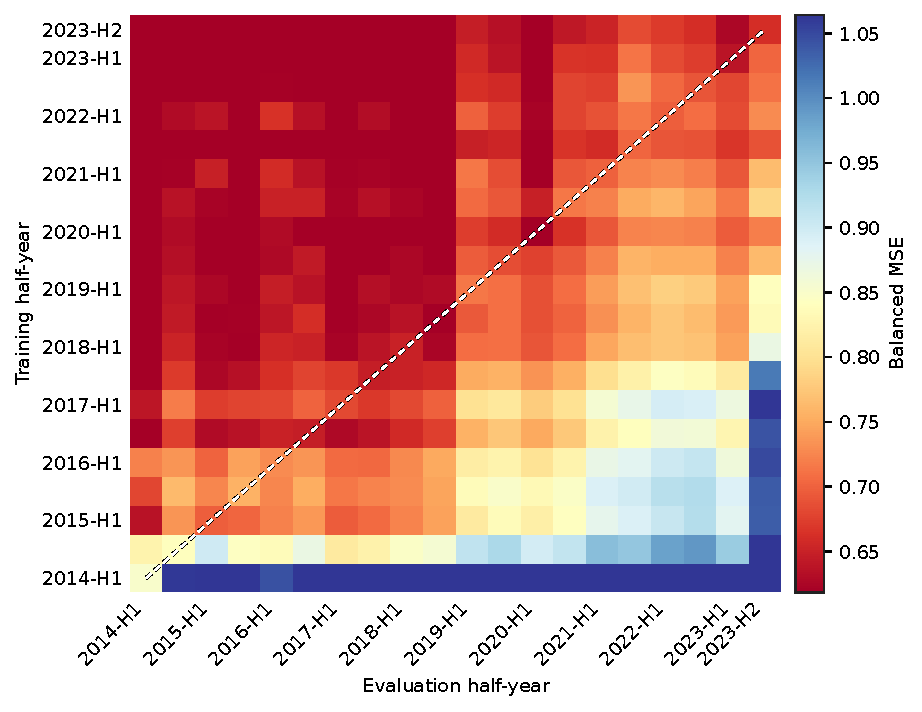
\includegraphics[width=0.49\linewidth]{plots_experiments/amazon_reviews/raw/BiLSTM-M_drift_matrix.pdf}\hfill
    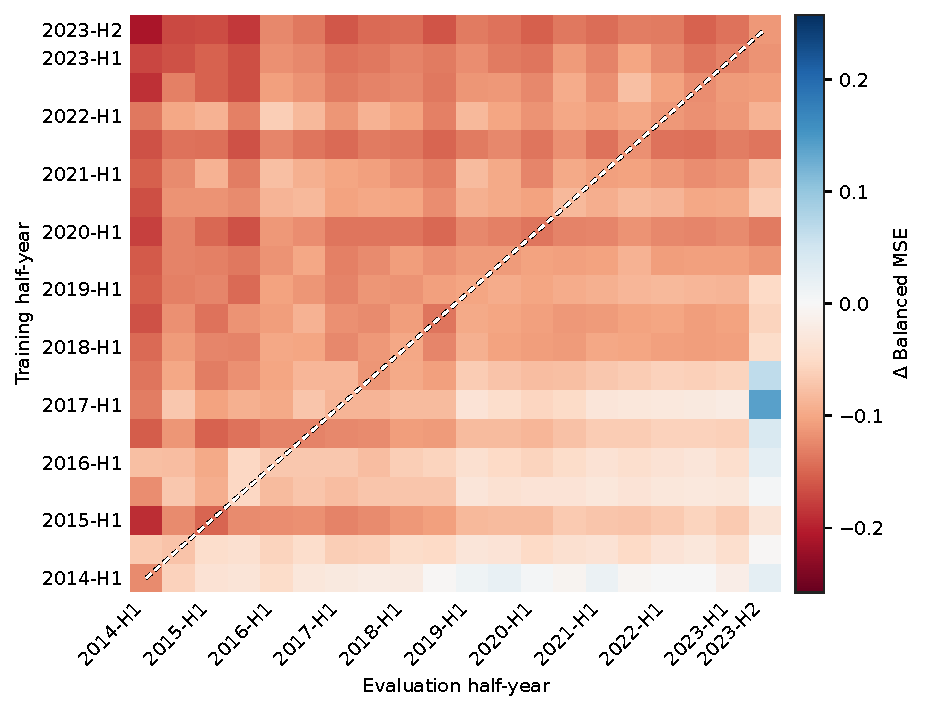
\includegraphics[width=0.49\linewidth]{plots_experiments/amazon_reviews/deviation/BiLSTM-M_deviation.pdf}
    \caption{BiLSTM-M}
    \label{fig:amazon_reviews_BiLSTM_M}
\end{subfigure}

\begin{subfigure}[t]{0.49\textwidth}\centering
    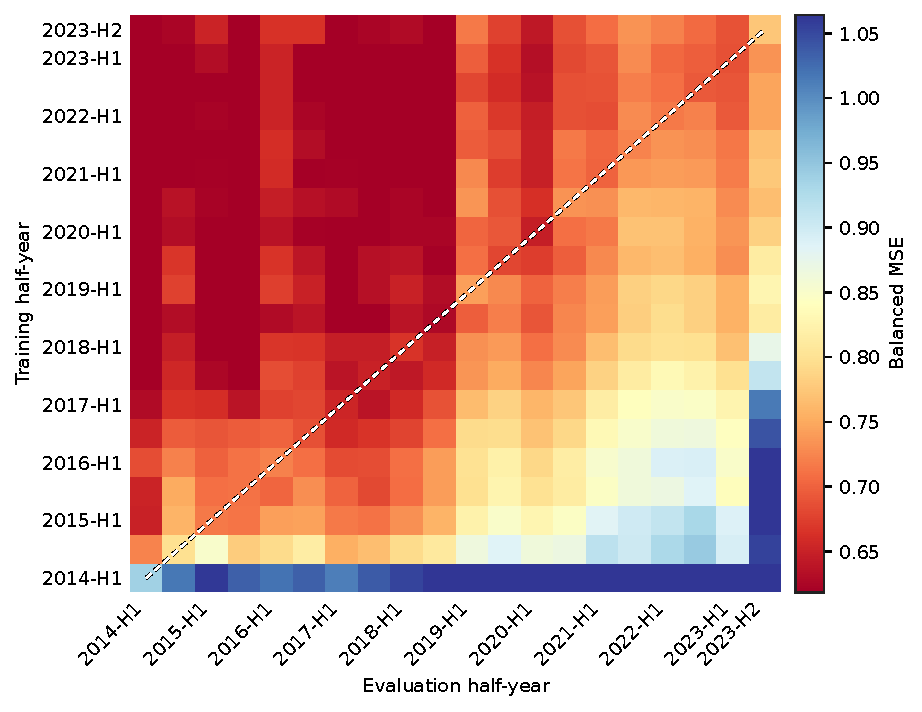
\includegraphics[width=0.49\linewidth]{plots_experiments/amazon_reviews/raw/BiLSTM-Attn-L_drift_matrix.pdf}\hfill
    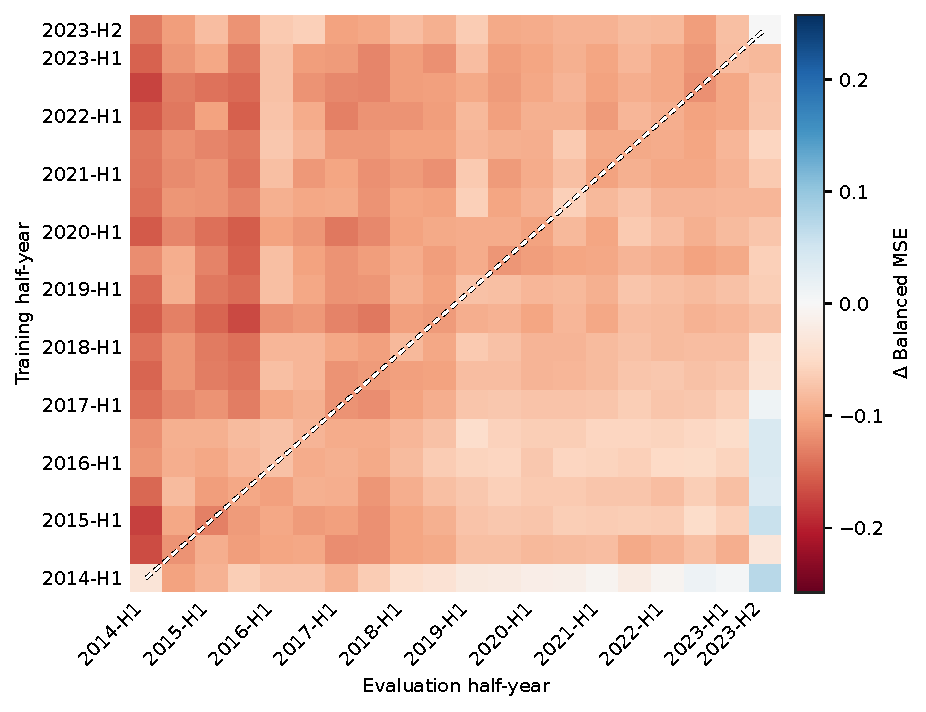
\includegraphics[width=0.49\linewidth]{plots_experiments/amazon_reviews/deviation/BiLSTM-Attn-L_deviation.pdf}
    \caption{BiLSTM-Attn-L}
    \label{fig:amazon_reviews_BiLSTM_Attn_L}
\end{subfigure}
\caption{Recurrent models: Balanced MSE drift matrix $M^{(m)}$ and deviation from the cohort mean $\Delta^{(m)} = M^{(m)} - \bar{M}$ for each model, shown on a sequential and a zero-centred diverging scale, respectively.}
\label{fig:amazon_reviews_family_text_rnn_regression}
\end{figure}

\subsection{Transformer}

\begin{figure}[H]
\centering
\begin{subfigure}[t]{0.49\textwidth}\centering
    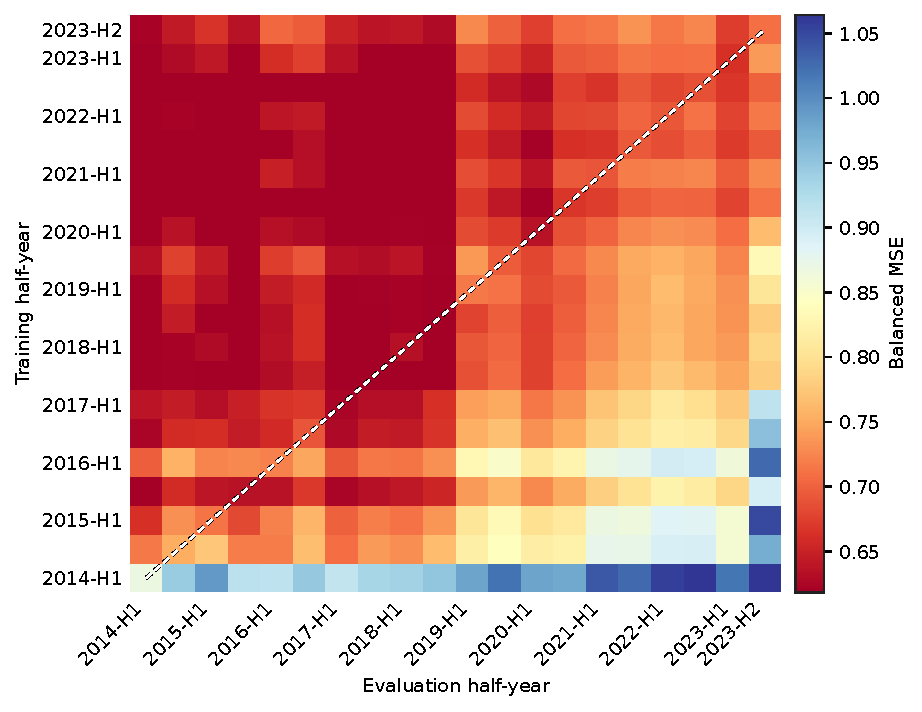
\includegraphics[width=0.49\linewidth]{plots_experiments/amazon_reviews/raw/TX-S_drift_matrix.pdf}\hfill
    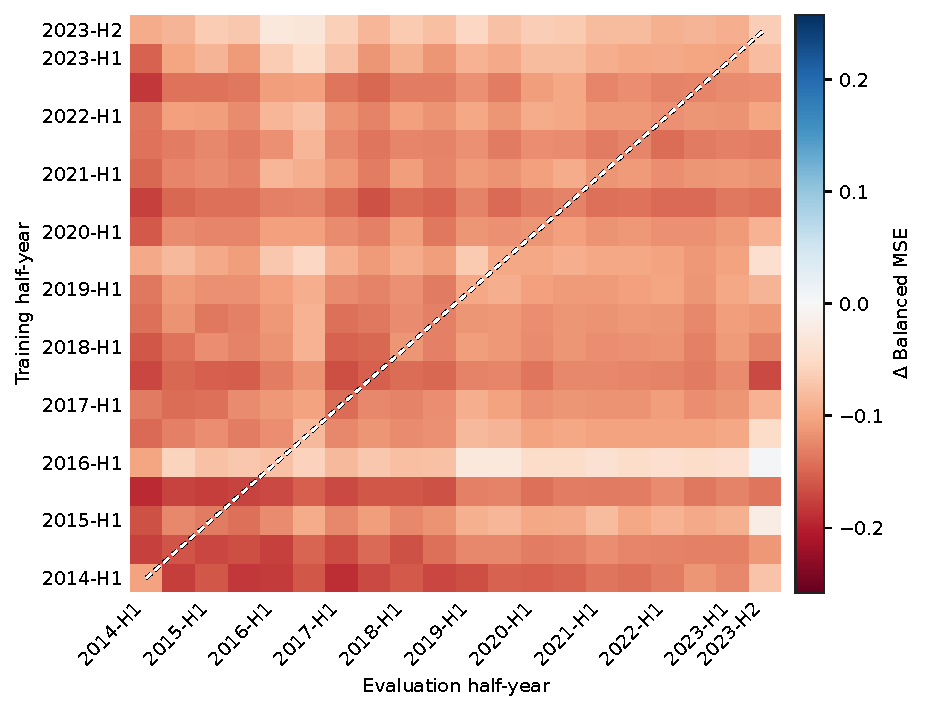
\includegraphics[width=0.49\linewidth]{plots_experiments/amazon_reviews/deviation/TX-S_deviation.pdf}
    \caption{TX-S}
    \label{fig:amazon_reviews_TX_S}
\end{subfigure}
\hfill
\begin{subfigure}[t]{0.49\textwidth}\centering
    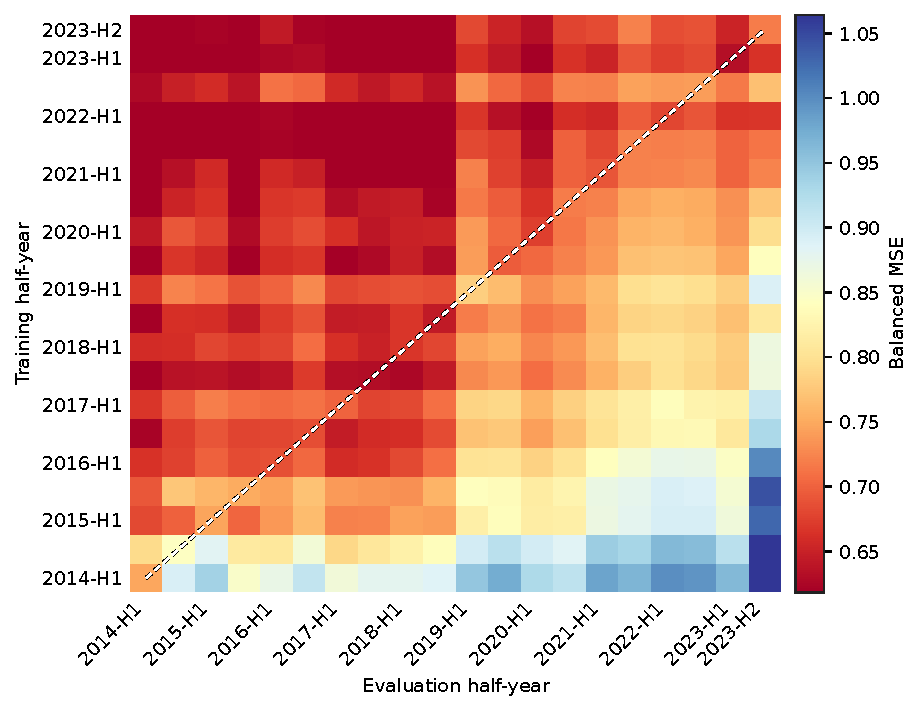
\includegraphics[width=0.49\linewidth]{plots_experiments/amazon_reviews/raw/TX-M_drift_matrix.pdf}\hfill
    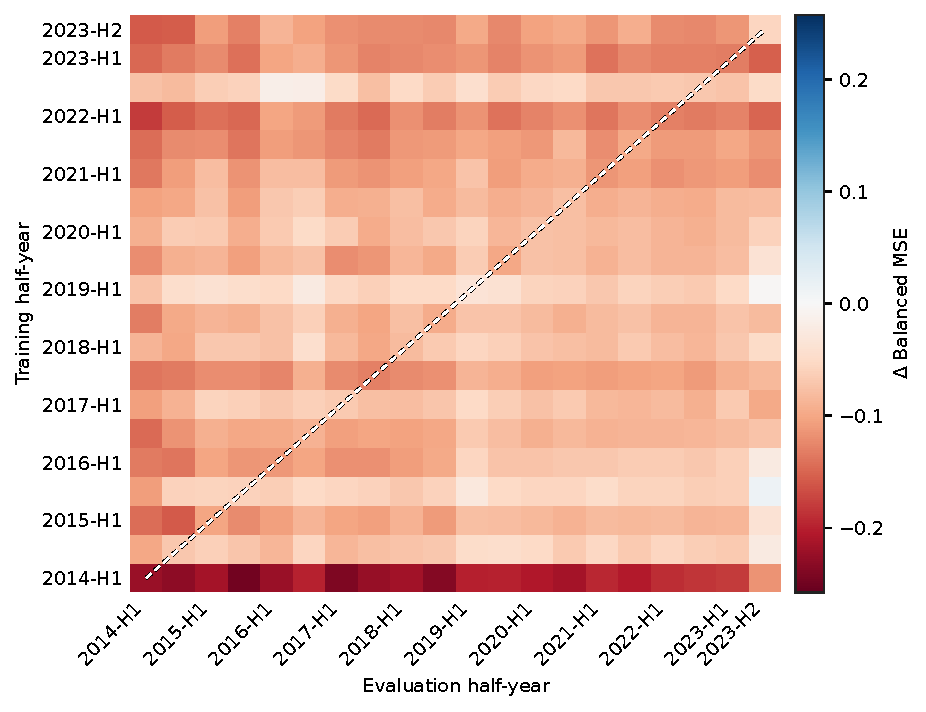
\includegraphics[width=0.49\linewidth]{plots_experiments/amazon_reviews/deviation/TX-M_deviation.pdf}
    \caption{TX-M}
    \label{fig:amazon_reviews_TX_M}
\end{subfigure}

\begin{subfigure}[t]{0.49\textwidth}\centering
    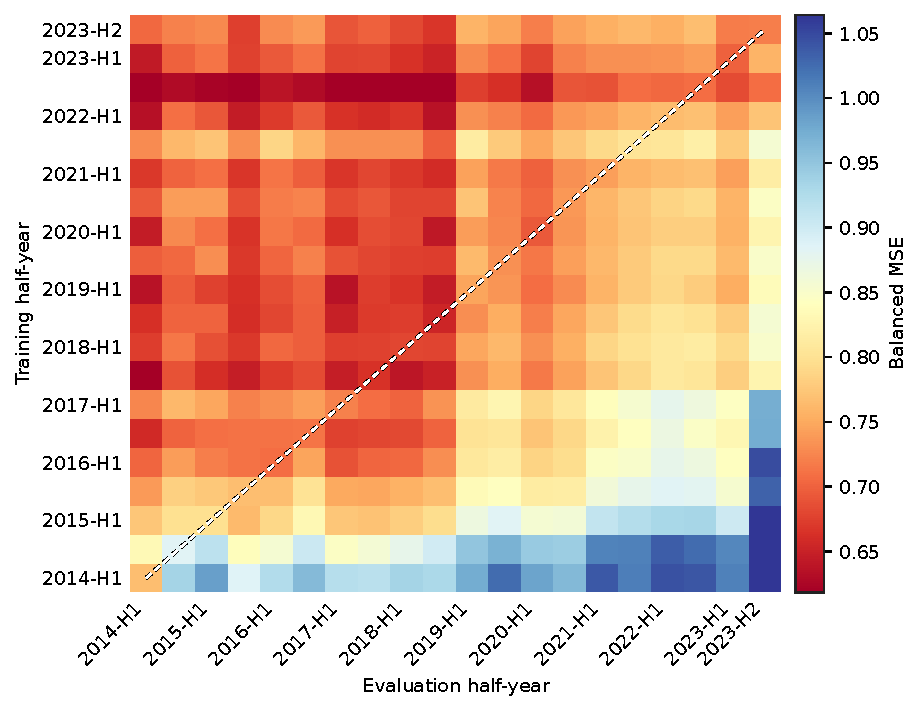
\includegraphics[width=0.49\linewidth]{plots_experiments/amazon_reviews/raw/TX-L_drift_matrix.pdf}\hfill
    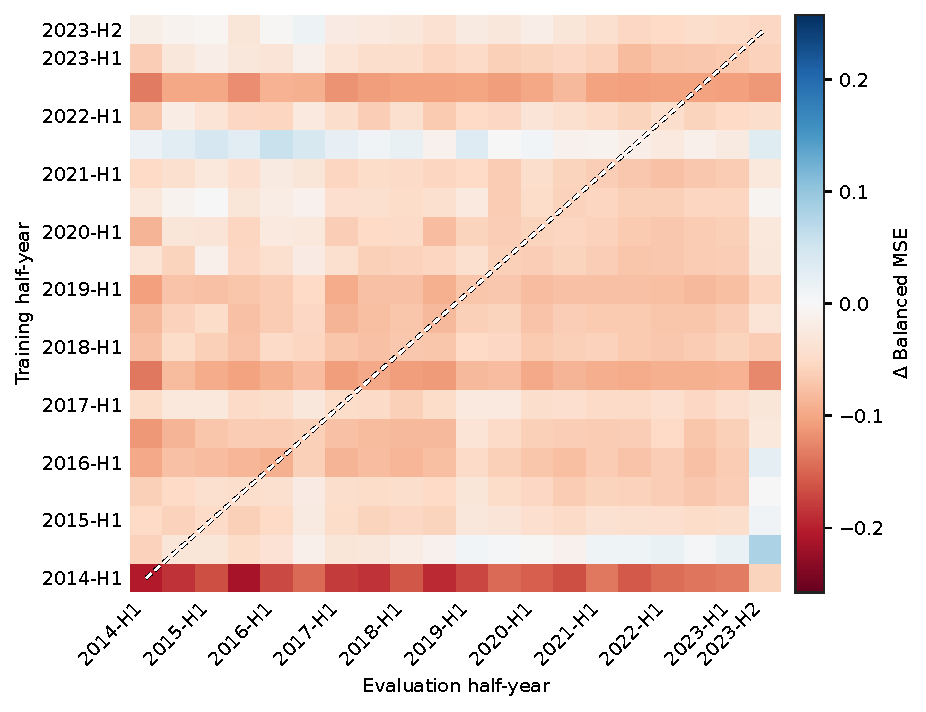
\includegraphics[width=0.49\linewidth]{plots_experiments/amazon_reviews/deviation/TX-L_deviation.pdf}
    \caption{TX-L}
    \label{fig:amazon_reviews_TX_L}
\end{subfigure}
\caption{Transformer models: Balanced MSE drift matrix $M^{(m)}$ and deviation from the cohort mean $\Delta^{(m)} = M^{(m)} - \bar{M}$ for each model, shown on a sequential and a zero-centred diverging scale, respectively.}
\label{fig:amazon_reviews_family_text_tx_regression}
\end{figure}

\subsection{Frozen}

\begin{figure}[H]
\centering
\begin{subfigure}[t]{0.49\textwidth}\centering
    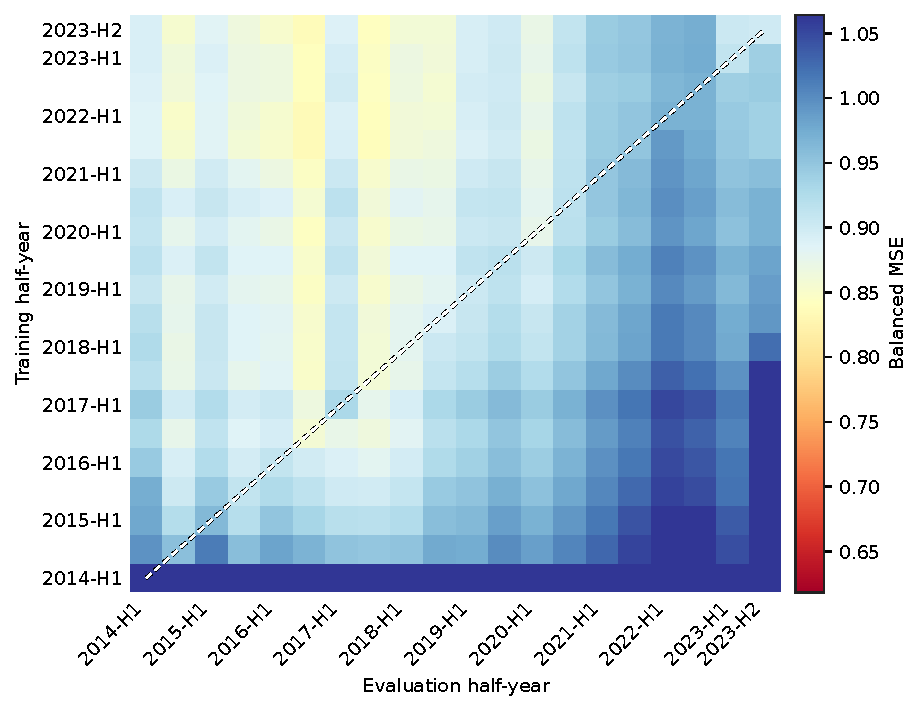
\includegraphics[width=0.49\linewidth]{plots_experiments/amazon_reviews/raw/BERT_drift_matrix.pdf}\hfill
    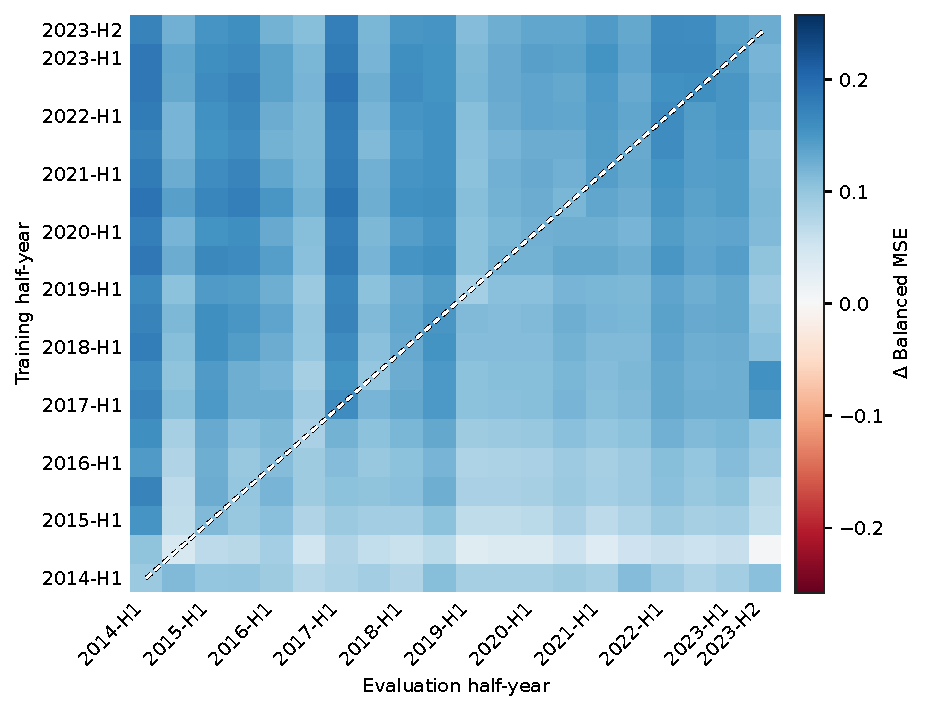
\includegraphics[width=0.49\linewidth]{plots_experiments/amazon_reviews/deviation/BERT_deviation.pdf}
    \caption{BERT}
    \label{fig:amazon_reviews_BERT}
\end{subfigure}
\hfill
\begin{subfigure}[t]{0.49\textwidth}\centering
    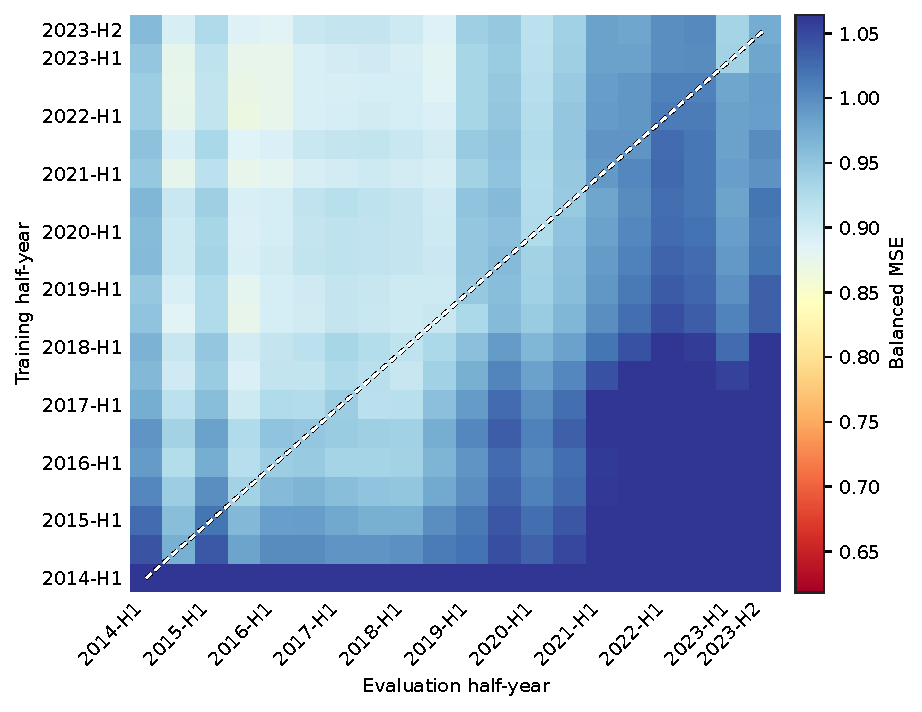
\includegraphics[width=0.49\linewidth]{plots_experiments/amazon_reviews/raw/DistilBERT_drift_matrix.pdf}\hfill
    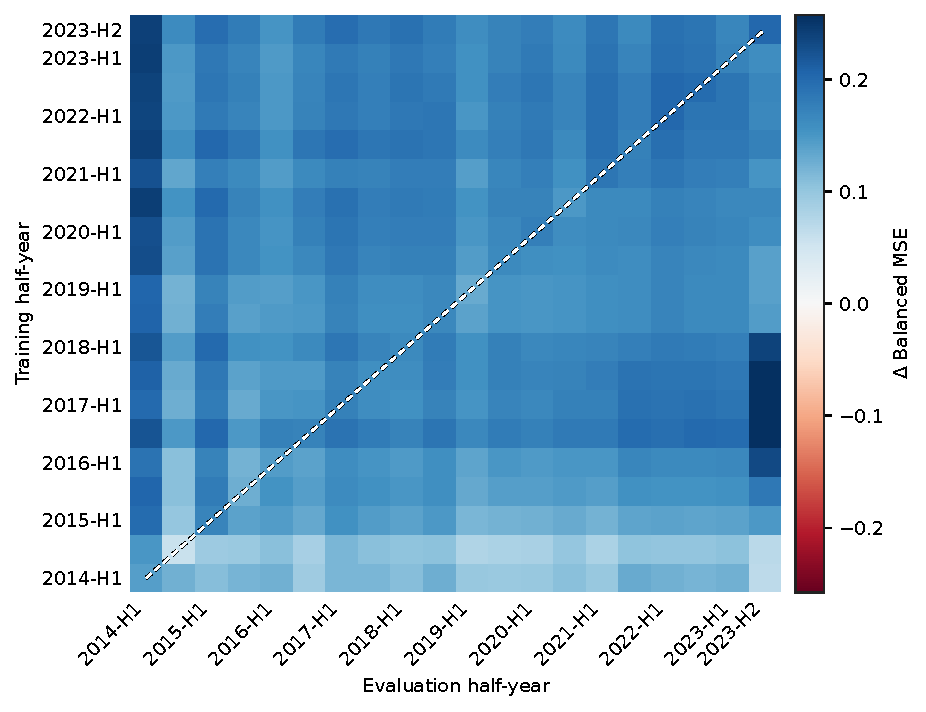
\includegraphics[width=0.49\linewidth]{plots_experiments/amazon_reviews/deviation/DistilBERT_deviation.pdf}
    \caption{DistilBERT}
    \label{fig:amazon_reviews_DistilBERT}
\end{subfigure}

\begin{subfigure}[t]{0.49\textwidth}\centering
    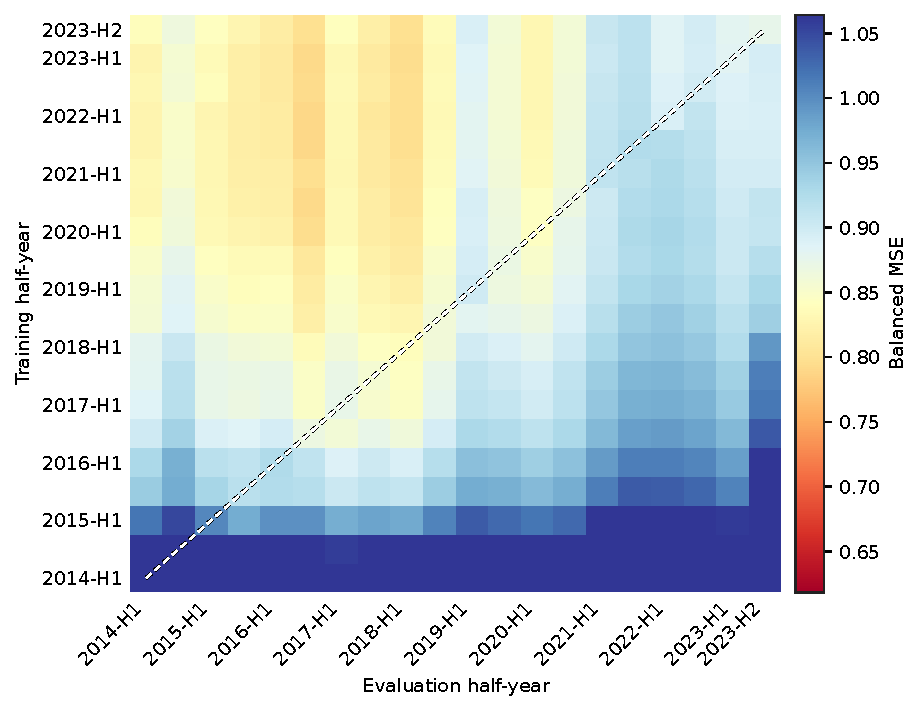
\includegraphics[width=0.49\linewidth]{plots_experiments/amazon_reviews/raw/ELECTRA_drift_matrix.pdf}\hfill
    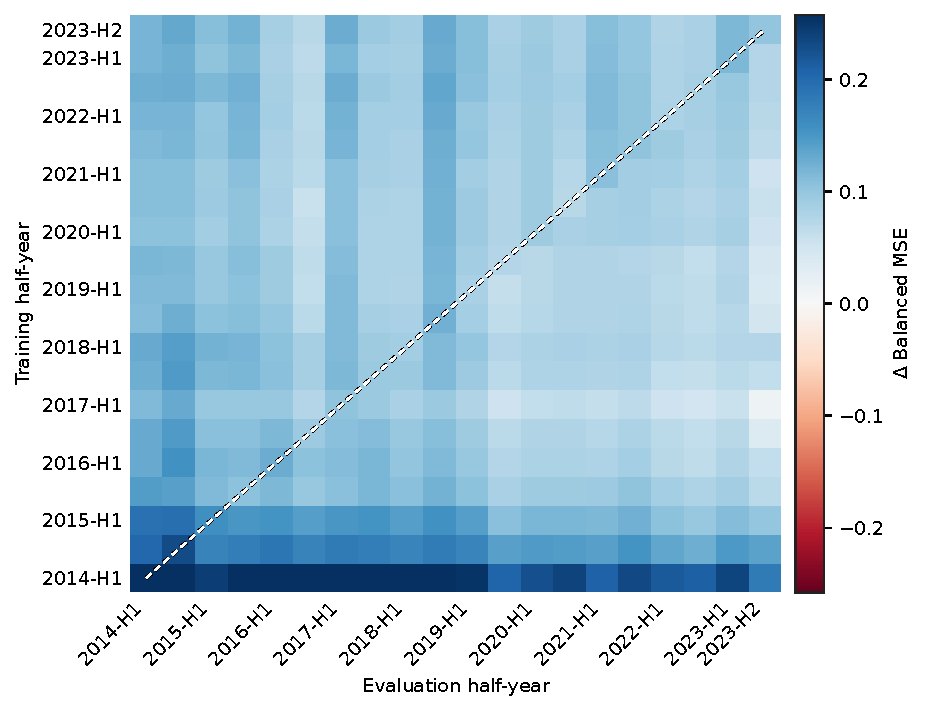
\includegraphics[width=0.49\linewidth]{plots_experiments/amazon_reviews/deviation/ELECTRA_deviation.pdf}
    \caption{ELECTRA}
    \label{fig:amazon_reviews_ELECTRA}
\end{subfigure}
\hfill
\begin{subfigure}[t]{0.49\textwidth}\centering
    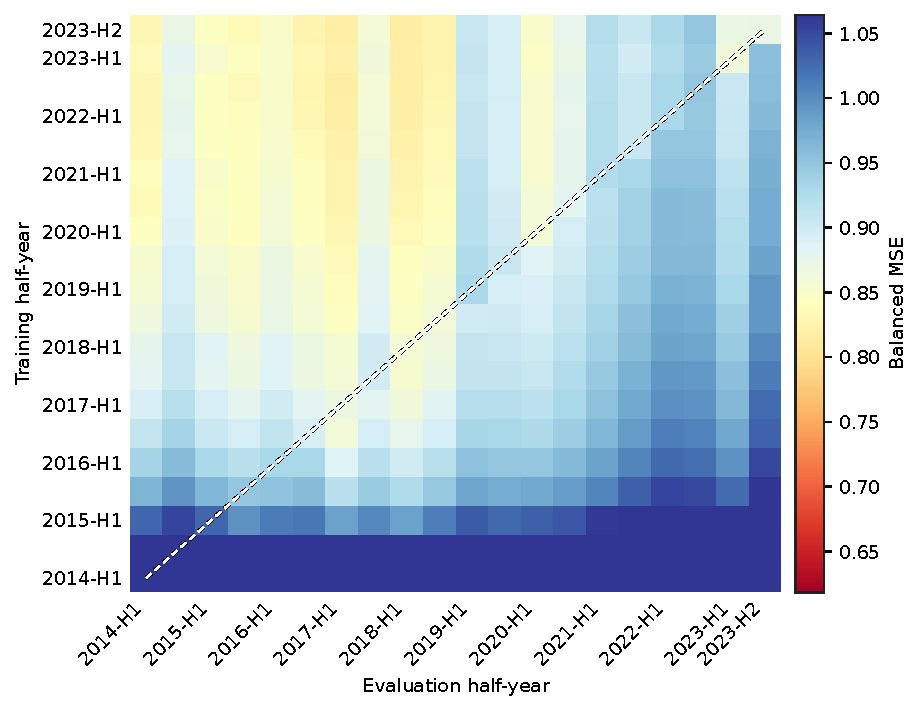
\includegraphics[width=0.49\linewidth]{plots_experiments/amazon_reviews/raw/MPNet_drift_matrix.pdf}\hfill
    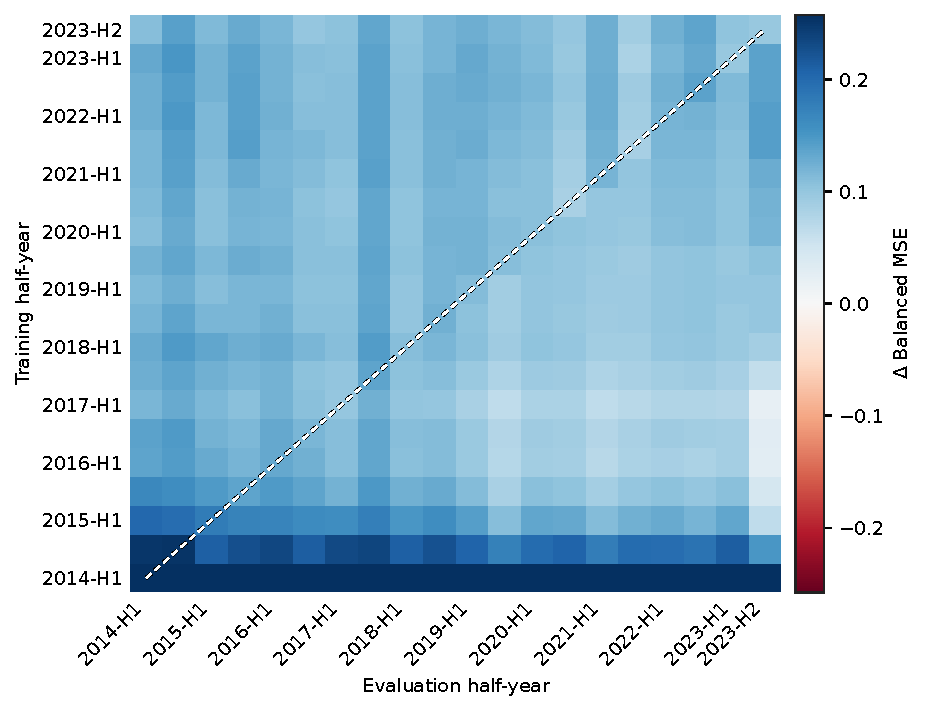
\includegraphics[width=0.49\linewidth]{plots_experiments/amazon_reviews/deviation/MPNet_deviation.pdf}
    \caption{MPNet}
    \label{fig:amazon_reviews_MPNet}
\end{subfigure}

\begin{subfigure}[t]{0.49\textwidth}\centering
    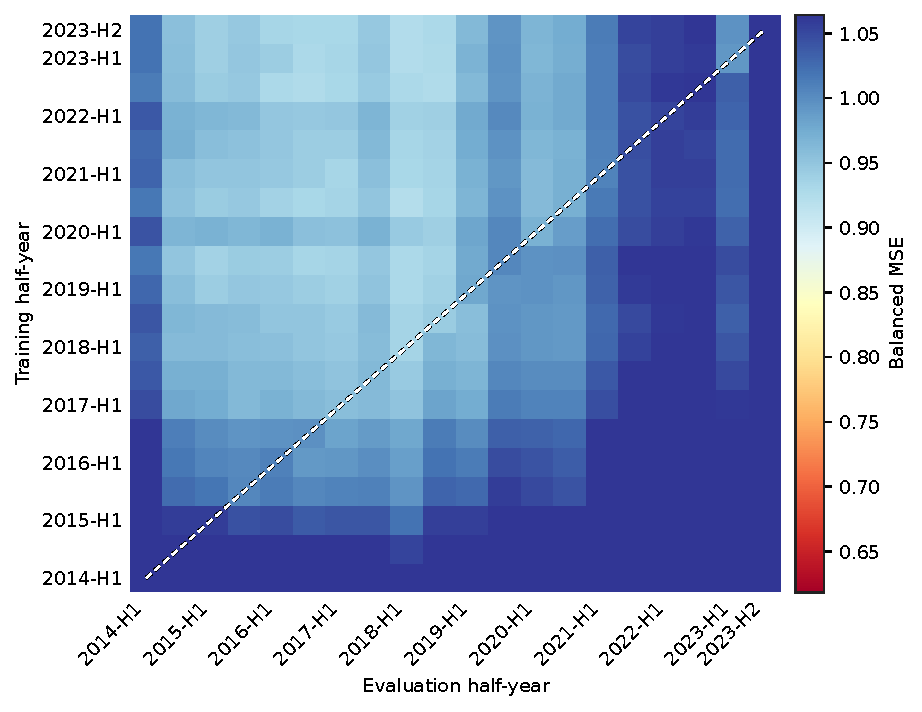
\includegraphics[width=0.49\linewidth]{plots_experiments/amazon_reviews/raw/ModernBERT_drift_matrix.pdf}\hfill
    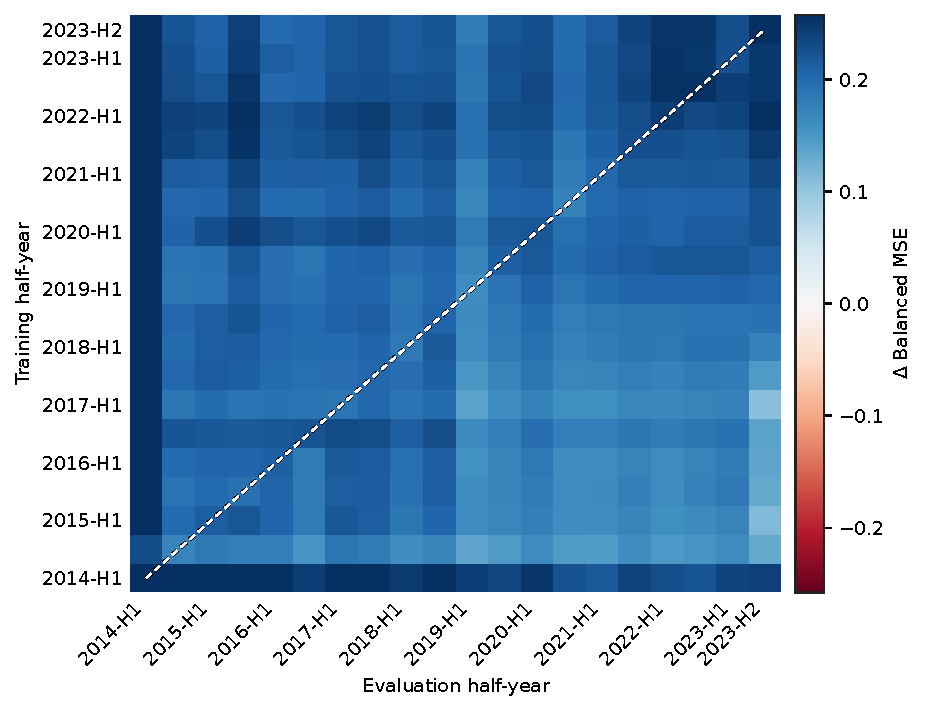
\includegraphics[width=0.49\linewidth]{plots_experiments/amazon_reviews/deviation/ModernBERT_deviation.pdf}
    \caption{ModernBERT}
    \label{fig:amazon_reviews_ModernBERT}
\end{subfigure}
\hfill
\begin{subfigure}[t]{0.49\textwidth}\centering
    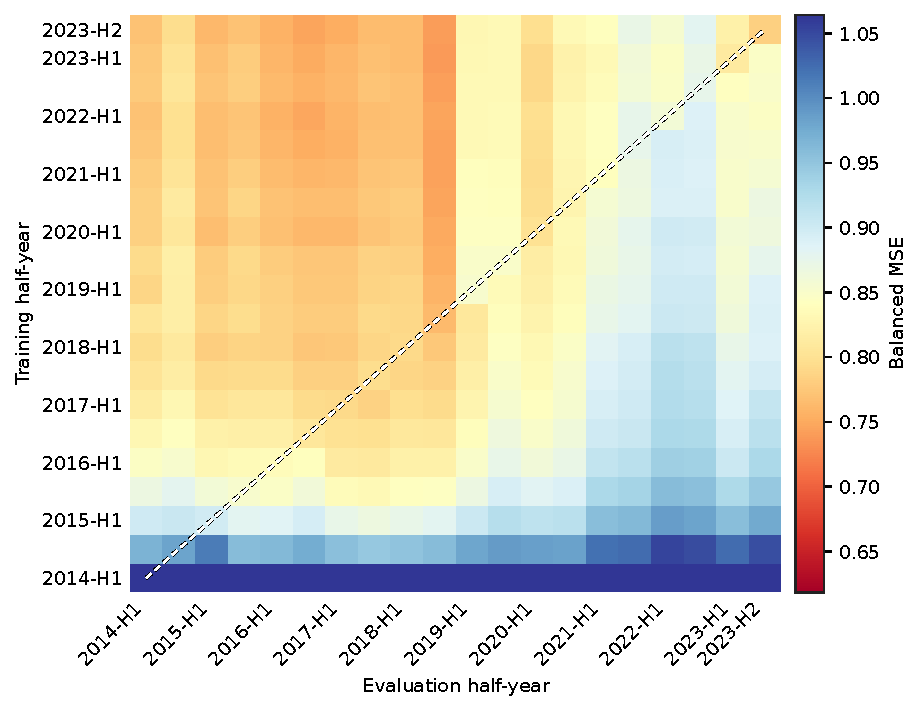
\includegraphics[width=0.49\linewidth]{plots_experiments/amazon_reviews/raw/RoBERTa_drift_matrix.pdf}\hfill
    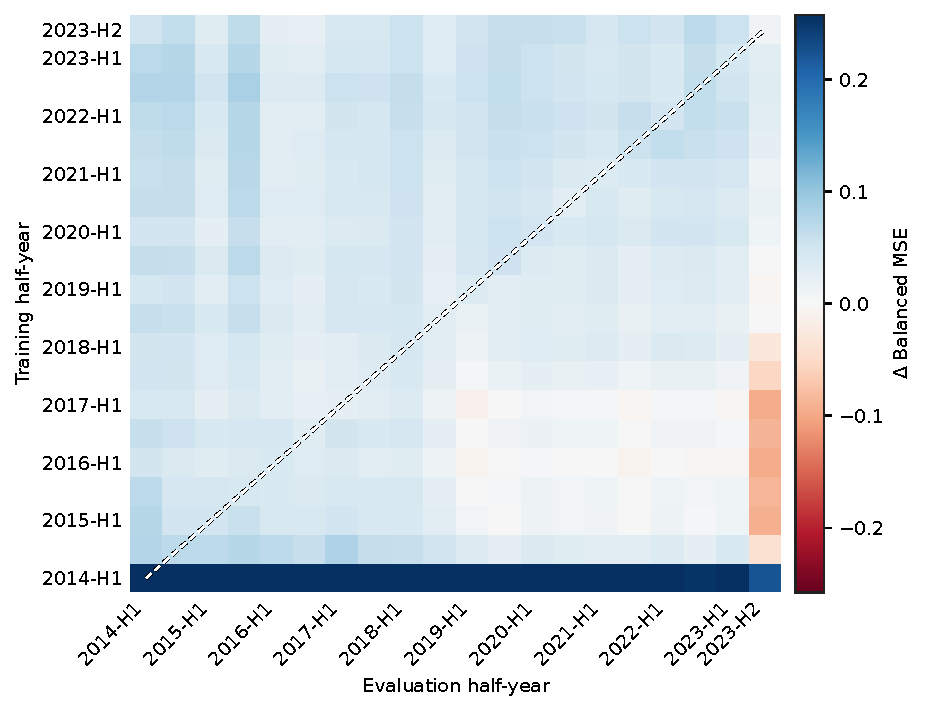
\includegraphics[width=0.49\linewidth]{plots_experiments/amazon_reviews/deviation/RoBERTa_deviation.pdf}
    \caption{RoBERTa}
    \label{fig:amazon_reviews_RoBERTa}
\end{subfigure}

\begin{subfigure}[t]{0.49\textwidth}\centering
    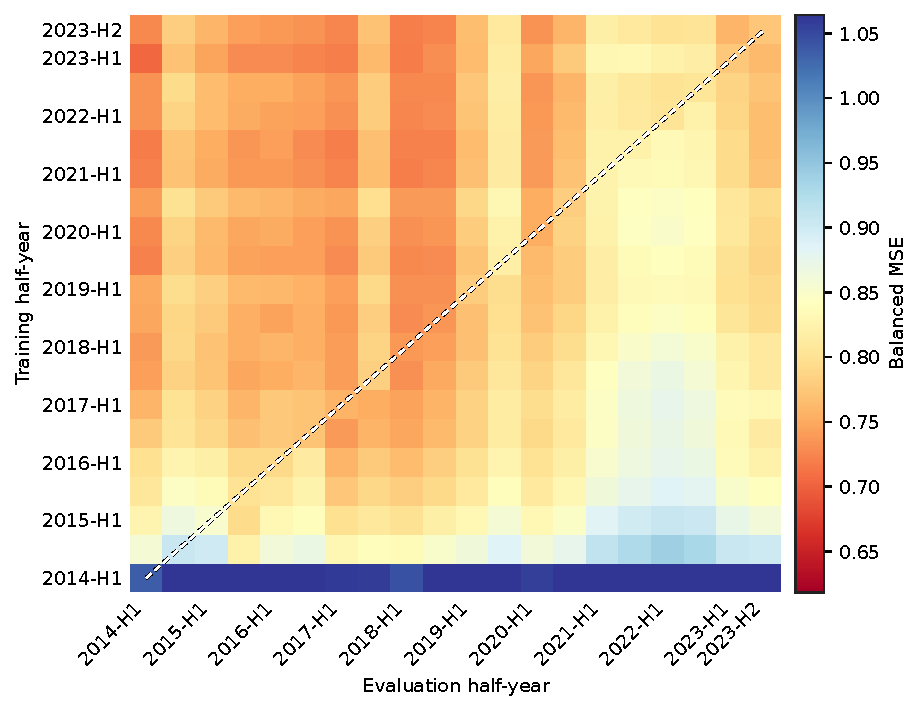
\includegraphics[width=0.49\linewidth]{plots_experiments/amazon_reviews/raw/DeBERTa-v3_drift_matrix.pdf}\hfill
    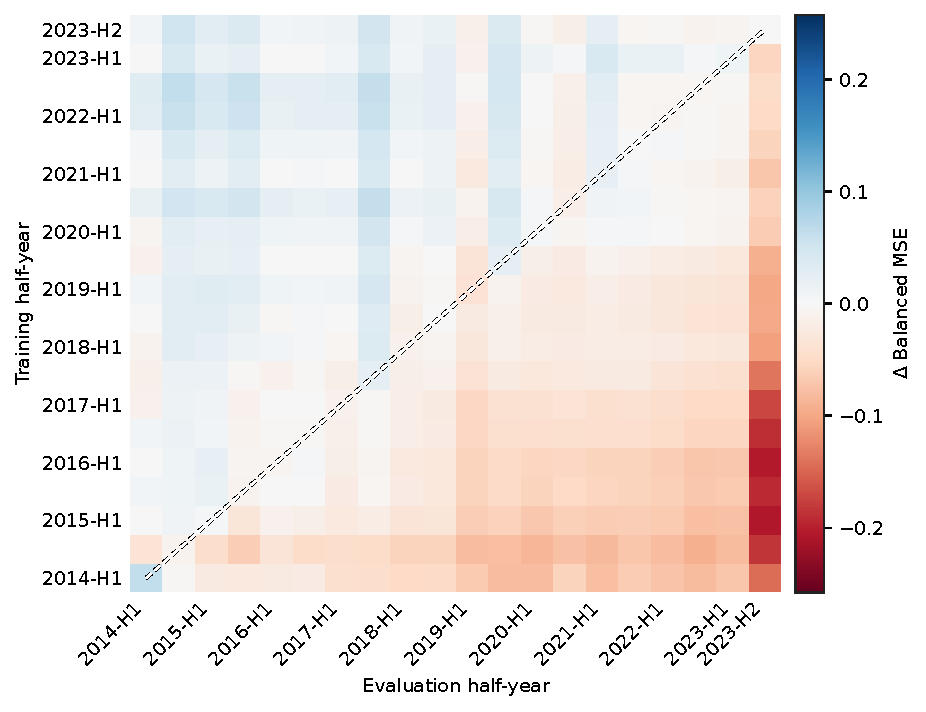
\includegraphics[width=0.49\linewidth]{plots_experiments/amazon_reviews/deviation/DeBERTa-v3_deviation.pdf}
    \caption{DeBERTa-v3}
    \label{fig:amazon_reviews_DeBERTa_v3}
\end{subfigure}
\caption{Frozen models: Balanced MSE drift matrix $M^{(m)}$ and deviation from the cohort mean $\Delta^{(m)} = M^{(m)} - \bar{M}$ for each model, shown on a sequential and a zero-centred diverging scale, respectively.}
\label{fig:amazon_reviews_family_text_frozen_head_regression}
\end{figure}

\subsection{Forgetting and Rankings}
\label{app:amazon_reviews_forgetting}

\noindent To see how quickly each model forgets, we summarize its drift matrix as a forgetting curve. The curve plots the Balanced MSE against the lag $\ell = j - i$, the number of slices between the training cutoff $i$ and the evaluation slice $j$. At each lag we average over all training cutoffs,
\[ F(\ell) = \operatorname{mean}_{i} M_{i,\,i+\ell}. \]
The result is the Balanced MSE at a fixed temporal distance, independent of which period a model was trained on. This separates the effect of temporal distance from the difficulty of any single slice.

\begin{figure}[H]
\centering
\begin{subfigure}[t]{0.49\textwidth}\centering
    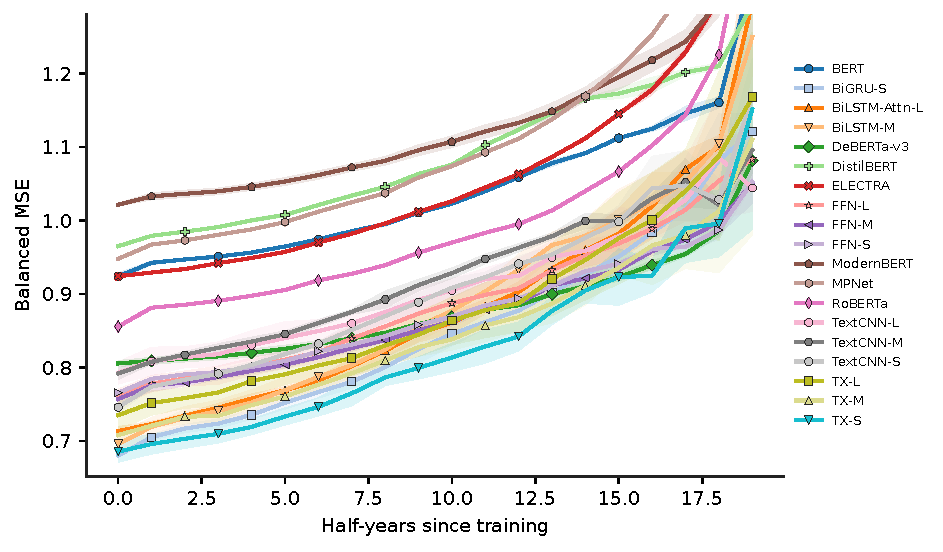
\includegraphics[width=\linewidth]{plots_experiments/amazon_reviews/forgetting.pdf}
    \caption{Per model}
    \label{fig:amazon_reviews_forgetting}
\end{subfigure}\hfill
\begin{subfigure}[t]{0.49\textwidth}\centering
    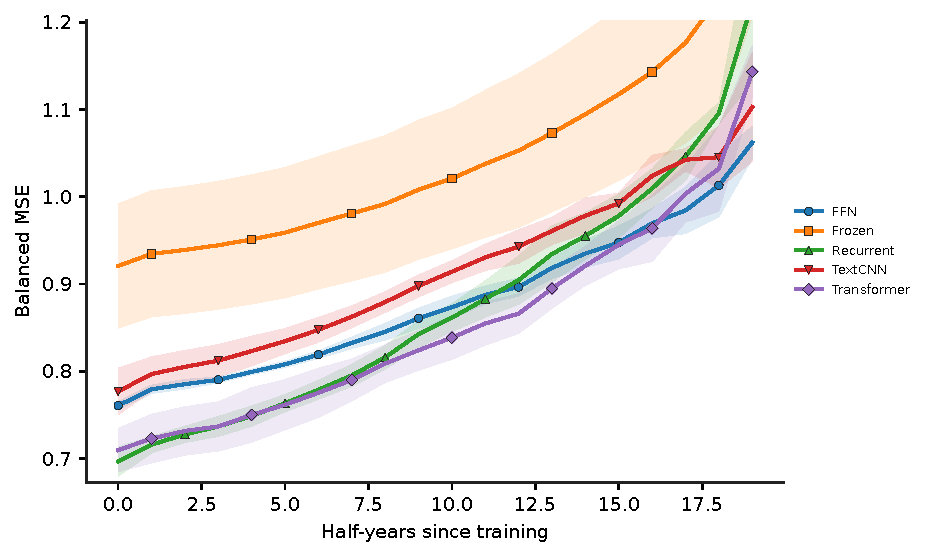
\includegraphics[width=\linewidth]{plots_experiments/amazon_reviews/forgetting_by_family.pdf}
    \caption{Per model family}
    \label{fig:amazon_reviews_forgetting_family}
\end{subfigure}
\caption{Forgetting curves: each model (left) and averaged within each family (right).}
\label{fig:amazon_reviews_forgetting_combined}
\end{figure}

\begin{figure}[H]
\centering
\begin{subfigure}[t]{0.49\textwidth}\centering
    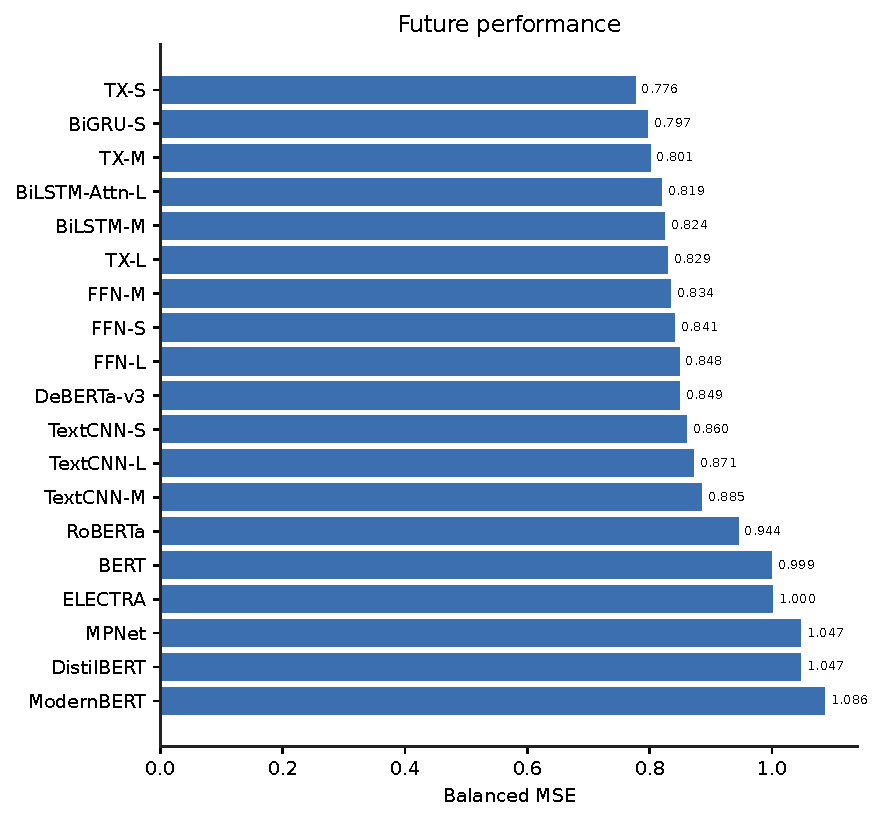
\includegraphics[width=\linewidth]{plots_experiments/amazon_reviews/ranking_future_performance.pdf}
    \caption{By future performance}
    \label{fig:amazon_reviews_ranking_future}
\end{subfigure}\hfill
\begin{subfigure}[t]{0.49\textwidth}\centering
    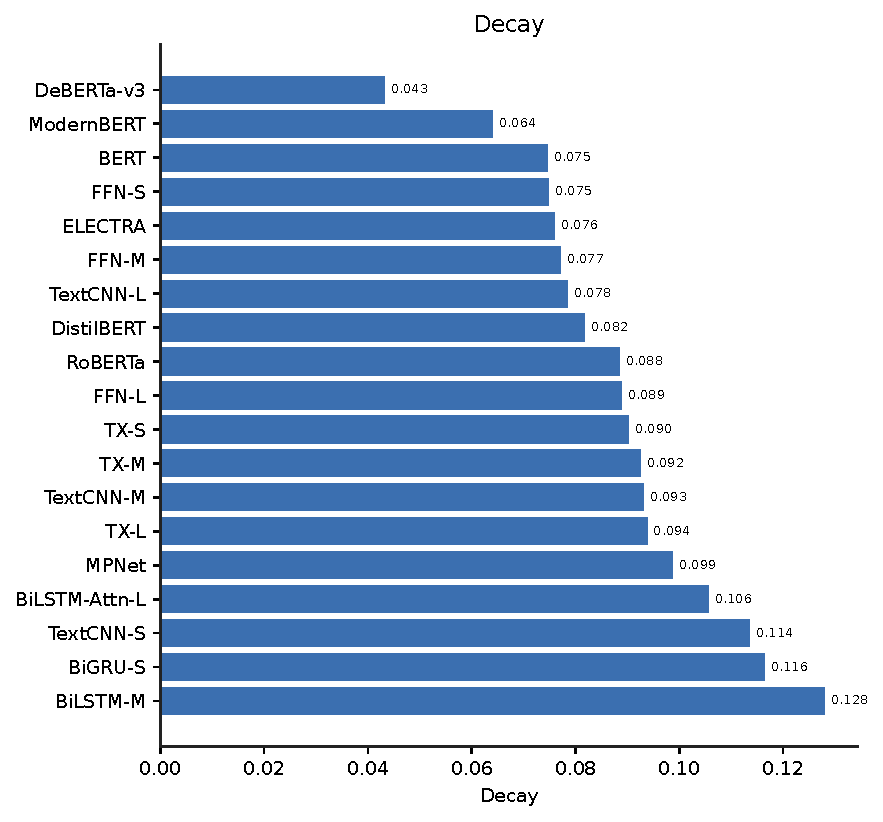
\includegraphics[width=\linewidth]{plots_experiments/amazon_reviews/ranking_decay.pdf}
    \caption{By decay}
    \label{fig:amazon_reviews_ranking_decay}
\end{subfigure}
\caption{Models ranked by mean future performance and by temporal decay.}
\label{fig:amazon_reviews_rankings}
\end{figure}

\subsection{Result Tables}

\begin{table}[H]
\centering
\footnotesize
\caption{Temporal robustness on Amazon Reviews.}
\label{tab:robustness_amazon_reviews}
\begin{minipage}[t]{0.49\linewidth}
\centering
\resizebox{\ifdim\width>\linewidth \linewidth\else\width\fi}{!}{%
\begin{tabular}{l rr}
\toprule
Model & Future & Decay \\
\midrule
DeBERTa-v3 & 0.849 & 0.043 \\
ModernBERT & 1.086 & 0.064 \\
BERT & 0.999 & 0.075 \\
FFN-S & 0.841 & 0.075 \\
ELECTRA & 1.000 & 0.076 \\
FFN-M & 0.834 & 0.077 \\
TextCNN-L & 0.871 & 0.078 \\
DistilBERT & 1.047 & 0.082 \\
RoBERTa & 0.944 & 0.088 \\
FFN-L & 0.848 & 0.089 \\
\bottomrule
\end{tabular}}
\end{minipage}\hfill
\begin{minipage}[t]{0.49\linewidth}
\centering
\resizebox{\ifdim\width>\linewidth \linewidth\else\width\fi}{!}{%
\begin{tabular}{l rr}
\toprule
Model & Future & Decay \\
\midrule
TX-S & 0.776 & 0.090 \\
TX-M & 0.801 & 0.092 \\
TextCNN-M & 0.885 & 0.093 \\
TX-L & 0.829 & 0.094 \\
MPNet & 1.047 & 0.099 \\
BiLSTM-Attn-L & 0.819 & 0.106 \\
TextCNN-S & 0.860 & 0.114 \\
BiGRU-S & 0.797 & 0.116 \\
BiLSTM-M & 0.824 & 0.128 \\
\bottomrule
\end{tabular}}
\end{minipage}
\end{table}


\noindent
\begin{minipage}[t]{0.49\linewidth}
\centering
\scriptsize
\setlength{\tabcolsep}{4pt}
\captionof{table}{Amazon Reviews: models trained up to 2014-H1, ordered by future performance.}
\label{tab:amazon_reviews_cutoff_28}
\resizebox{\ifdim\width>\linewidth \linewidth\else\width\fi}{!}{%
\begin{tabular}{c l rrr}
\toprule
Rank & Model & Balanced MSE & Future & Decay \\
\midrule
1 & TX-M & 0.748 & 0.933 & 0.185 \\
2 & TextCNN-L & 0.782 & 0.935 & 0.153 \\
3 & FFN-L & 0.836 & 0.972 & 0.136 \\
4 & TX-L & 0.767 & 0.981 & 0.215 \\
5 & FFN-M & 0.885 & 0.986 & 0.100 \\
6 & TX-S & 0.868 & 0.987 & 0.119 \\
7 & TextCNN-M & 0.761 & 0.993 & 0.231 \\
8 & FFN-S & 0.907 & 1.023 & 0.116 \\
9 & BiGRU-S & 0.790 & 1.073 & 0.283 \\
10 & TextCNN-S & 0.782 & 1.078 & 0.296 \\
11 & DeBERTa-v3 & 1.035 & 1.083 & 0.048 \\
12 & BiLSTM-Attn-L & 0.938 & 1.105 & 0.167 \\
13 & BiLSTM-M & 0.850 & 1.127 & 0.277 \\
14 & BERT & 1.067 & 1.232 & 0.165 \\
15 & DistilBERT & 1.113 & 1.250 & 0.137 \\
16 & ELECTRA & 1.332 & 1.382 & 0.050 \\
17 & ModernBERT & 1.273 & 1.386 & 0.113 \\
18 & RoBERTa & 1.227 & 1.468 & 0.241 \\
19 & MPNet & 1.492 & 1.657 & 0.165 \\
\bottomrule
\end{tabular}}
\end{minipage}
\hfill
\begin{minipage}[t]{0.49\linewidth}
\centering
\scriptsize
\setlength{\tabcolsep}{4pt}
\captionof{table}{Amazon Reviews: models trained up to 2017-H1, ordered by future performance.}
\label{tab:amazon_reviews_cutoff_34}
\resizebox{\ifdim\width>\linewidth \linewidth\else\width\fi}{!}{%
\begin{tabular}{c l rrr}
\toprule
Rank & Model & Balanced MSE & Future & Decay \\
\midrule
1 & TX-S & 0.625 & 0.748 & 0.123 \\
2 & BiGRU-S & 0.644 & 0.765 & 0.121 \\
3 & TX-M & 0.701 & 0.785 & 0.084 \\
4 & BiLSTM-Attn-L & 0.654 & 0.789 & 0.136 \\
5 & FFN-L & 0.724 & 0.810 & 0.086 \\
6 & FFN-S & 0.723 & 0.812 & 0.089 \\
7 & DeBERTa-v3 & 0.758 & 0.814 & 0.056 \\
8 & TextCNN-S & 0.711 & 0.817 & 0.106 \\
9 & TX-L & 0.722 & 0.818 & 0.096 \\
10 & BiLSTM-M & 0.681 & 0.828 & 0.147 \\
11 & FFN-M & 0.742 & 0.829 & 0.087 \\
12 & RoBERTa & 0.792 & 0.860 & 0.068 \\
13 & TextCNN-L & 0.789 & 0.876 & 0.087 \\
14 & TextCNN-M & 0.773 & 0.885 & 0.113 \\
15 & ELECTRA & 0.873 & 0.926 & 0.052 \\
16 & MPNet & 0.868 & 0.940 & 0.072 \\
17 & BERT & 0.929 & 0.984 & 0.055 \\
18 & ModernBERT & 0.958 & 1.028 & 0.070 \\
19 & DistilBERT & 0.942 & 1.047 & 0.104 \\
\bottomrule
\end{tabular}}
\end{minipage}


\vspace{1.5ex}

\noindent
\begin{minipage}[t]{0.49\linewidth}
\centering
\scriptsize
\setlength{\tabcolsep}{4pt}
\captionof{table}{Amazon Reviews: models trained up to 2020-H1, ordered by future performance.}
\label{tab:amazon_reviews_cutoff_40}
\resizebox{\ifdim\width>\linewidth \linewidth\else\width\fi}{!}{%
\begin{tabular}{c l rrr}
\toprule
Rank & Model & Balanced MSE & Future & Decay \\
\midrule
1 & BiLSTM-M & 0.614 & 0.706 & 0.092 \\
2 & BiGRU-S & 0.627 & 0.715 & 0.088 \\
3 & TX-S & 0.637 & 0.721 & 0.084 \\
4 & BiLSTM-Attn-L & 0.647 & 0.749 & 0.102 \\
5 & TX-M & 0.675 & 0.751 & 0.076 \\
6 & TextCNN-S & 0.672 & 0.767 & 0.094 \\
7 & TX-L & 0.693 & 0.773 & 0.080 \\
8 & FFN-L & 0.713 & 0.793 & 0.080 \\
9 & FFN-S & 0.729 & 0.795 & 0.066 \\
10 & FFN-M & 0.744 & 0.817 & 0.074 \\
11 & DeBERTa-v3 & 0.753 & 0.820 & 0.067 \\
12 & TextCNN-M & 0.748 & 0.833 & 0.085 \\
13 & TextCNN-L & 0.743 & 0.834 & 0.091 \\
14 & RoBERTa & 0.800 & 0.870 & 0.070 \\
15 & ELECTRA & 0.844 & 0.911 & 0.067 \\
16 & MPNet & 0.860 & 0.938 & 0.078 \\
17 & BERT & 0.876 & 0.959 & 0.084 \\
18 & DistilBERT & 0.926 & 0.998 & 0.072 \\
19 & ModernBERT & 0.969 & 1.041 & 0.072 \\
\bottomrule
\end{tabular}}
\end{minipage}
\hfill
\begin{minipage}[t]{0.49\linewidth}
\centering
\scriptsize
\setlength{\tabcolsep}{4pt}
\captionof{table}{Amazon Reviews: models trained up to 2023-H1, ordered by future performance.}
\label{tab:amazon_reviews_cutoff_46}
\resizebox{\ifdim\width>\linewidth \linewidth\else\width\fi}{!}{%
\begin{tabular}{c l rrr}
\toprule
Rank & Model & Balanced MSE & Future & Decay \\
\midrule
1 & TX-M & 0.634 & 0.665 & 0.031 \\
2 & BiGRU-S & 0.627 & 0.691 & 0.064 \\
3 & BiLSTM-M & 0.638 & 0.703 & 0.065 \\
4 & BiLSTM-Attn-L & 0.687 & 0.735 & 0.048 \\
5 & TX-S & 0.663 & 0.740 & 0.077 \\
6 & TextCNN-S & 0.682 & 0.747 & 0.066 \\
7 & TX-L & 0.699 & 0.759 & 0.060 \\
8 & DeBERTa-v3 & 0.776 & 0.764 & -0.013 \\
9 & FFN-L & 0.728 & 0.770 & 0.042 \\
10 & FFN-S & 0.731 & 0.777 & 0.046 \\
11 & FFN-M & 0.742 & 0.821 & 0.079 \\
12 & TextCNN-M & 0.751 & 0.838 & 0.087 \\
13 & RoBERTa & 0.812 & 0.847 & 0.035 \\
14 & TextCNN-L & 0.794 & 0.869 & 0.075 \\
15 & ELECTRA & 0.882 & 0.894 & 0.012 \\
16 & BERT & 0.911 & 0.939 & 0.029 \\
17 & MPNet & 0.863 & 0.956 & 0.093 \\
18 & DistilBERT & 0.937 & 0.980 & 0.043 \\
19 & ModernBERT & 0.992 & 1.069 & 0.076 \\
\bottomrule
\end{tabular}}
\end{minipage}


\begin{table}[H]
\centering
\footnotesize
\caption{Amazon Reviews: future performance and decay by model family.}
\label{tab:amazon_reviews_by_family}
\begin{tabular}{l rrrrrrrr}
\toprule
 & \multicolumn{2}{c}{2014-H1} & \multicolumn{2}{c}{2017-H1} & \multicolumn{2}{c}{2020-H1} & \multicolumn{2}{c}{2023-H1} \\
Family & Future & Decay & Future & Decay & Future & Decay & Future & Decay \\
\midrule
FFN & 0.993 & 0.117 & 0.817 & 0.087 & 0.802 & 0.073 & 0.789 & 0.056 \\
Frozen & 1.351 & 0.131 & 0.943 & 0.068 & 0.934 & 0.073 & 0.921 & 0.039 \\
Recurrent & 1.101 & 0.242 & 0.794 & 0.134 & 0.723 & 0.094 & 0.710 & 0.059 \\
TextCNN & 1.002 & 0.227 & 0.859 & 0.102 & 0.811 & 0.090 & 0.818 & 0.076 \\
Transformer & 0.967 & 0.173 & 0.784 & 0.101 & 0.748 & 0.080 & 0.721 & 0.056 \\
\bottomrule
\end{tabular}
\end{table}

